\chapter{Sequence analysis of polarity in transmembrane helices suggests that translocation of marginally hydrophobic helices could be facilitated by neighbouring typically hydrophobic helices}
\chaptermark{Sequence analysis of polarity...}
\section{Abstract}

Marginally hydrophobic transmembrane helices perform a variety of essential for life intra-membrane molecular biochemistry.
However, due to their relatively polar composition, they often lack sufficient hydrophobicity by themselves to incorporate into the membrane efficiently via the translocon.
Other elements of the sequence context, such as other transmembrane helices or flexible loop regions, allow the marginally hydrophobic transmembrane regions to integrate into the membrane environment.
Here we analyse large numbers of multipass transmembrane protein sequences stratified by protein families and molecular functions to show that there are conserved stark differences between sequentially adjacent transmembrane helices in terms of hydrophobicity and TMSOC complexity.
Not all classes of transmembrane protein have these highly polar\--hydrophobic pairs.
In the instances of GPCRs and ion channels, there is evidence in the literature to support cooperative insertion between these highly polar\--hydrophobic transmembrane helix pairs highlighted in our results.


\section{Introduction}

Translocation is the process of incorporating a \gls{tmp} into the membrane.
A ribosome translates the~\gls{rna} to a nascent peptide chain which is handed directly (co-translational insertion) or indirectly (post\--translational insertion) to the translocon insertion machinery.
This translocon assembly then threads the chain through the membrane and releases hydrophobic~\gls{tmh}s into the membrane environment (Figure \ref{fig:sequential-insertion}).

\begin{figure}[!ht]
\centering
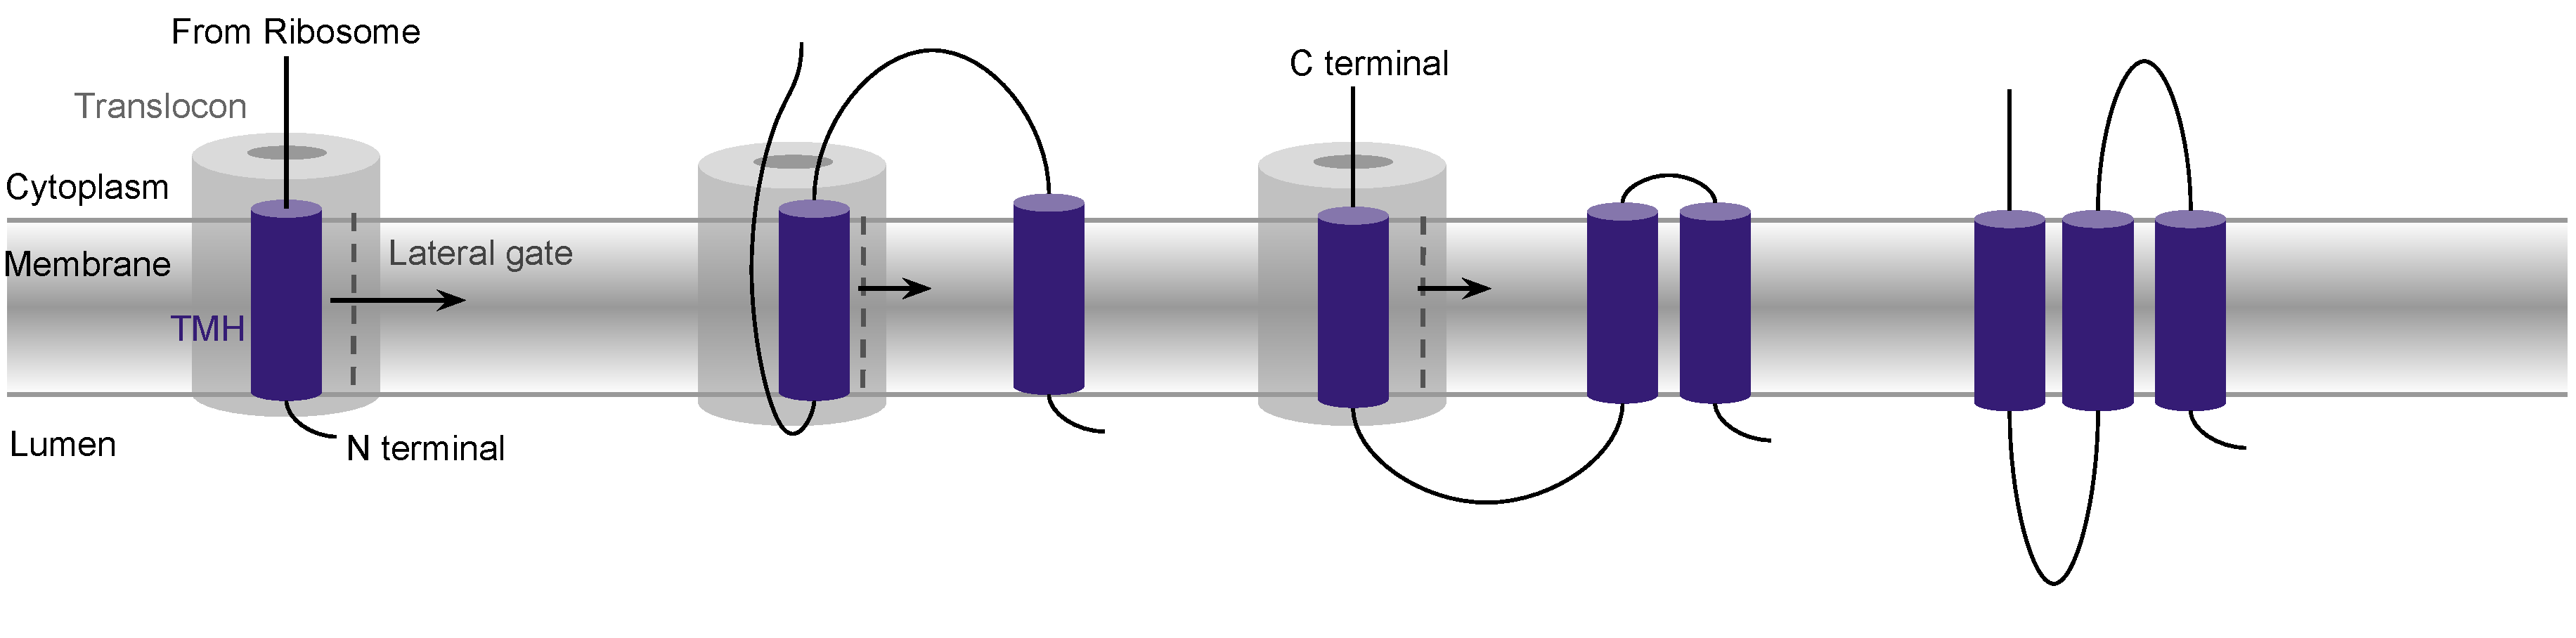
\includegraphics[width=1\textwidth]{multipass-folding/sequential-insertion}
        \captionof{figure}[A cartoon showing the generally accepted schematic of sequential multipass transmembrane helix insertion into the membranes.]{\textbf{A cartoon showing the generally accepted schematic of sequential multipass transmembrane helix insertion into the membranes.}
        The two key concepts are that one at a time, the TMHs emerge from the ribosome into the translocon.
        This appearance of hydrophobicity triggers the lateral gate to open.
        As the nascent TMH is exposed to the membrane, it begins to partition.
        The downstream protein from the TMH is then threaded through the translocon until the next TMH is recognised.
        This implies that the TMHs ultimately have no meaningful interactions with one another until the protein has been threaded into the membrane and the multiple TMHs form a bundle.
}
\label{fig:sequential-insertion}
\end{figure}

The overwhelming majority of~\gls{tmp}s use the co-translational method of translocation.
It has long been understood that this method is essentially the~\gls{srp} recognising and attaching to the nascent peptide chain whilst it is still associated with the ribosome, and the~\gls{srp} then targets the peptide and ribosome to an~\gls{sr} in association with the membrane insertion machinery on the~\gls{er} membrane~\cite{Pool2005, Hessa2005}.

Crystal structures showed the \gls{srp} targets the nascent peptide chain for membrane insertion via a GTPase in both the \gls{srp} and the membrane bound translocon associated \gls{sr} ~\cite{Shan2005}.
the \gls{srp}\--ribosome\--nascent peptide complex associates with the translocon\--\gls{sr} complex thus bringing the nascent peptide chain in proximity to the translocon~\cite{Shan2005}.
Mutant studies of \gls{srp} revealed key discrete conformational stages~\cite{Shan2005}.
These are the specific recognition of signal sequences on cargo proteins, the targeting of the package to the membrane, the handing over of the cargo to the translocation machinery all the while maintaining precise spatial and temporal coordination of each molecular event \cite{Saraogi2011}.

%NOPI rules

The prevailing view of membrane insertion by the translocon is that the \gls{tmh}s partition in the membrane one at a time as the translocon lateral gate opens, exposing the \gls{tmh} to the membrane (Figure \ref{fig:sequential-insertion})~\cite{Cymer2015}.

\subsection{The ribosome-translocon complex in the biogenesis of membrane proteins.}
Ribosomes translate mRNA sequences into amino acid chains and are present in all living cells, and indeed the ribosomal complexes presence and activity is considered an important distinction in biology between ribosome\--encoding organisms and capsid encoding organisms \cite{Raoult2008}.
They are a highly conserved \gls{rna}\--protein complex with a multitude of accessory proteins and targetting factors.

During translation of a \gls{tmp} protein, the \gls{srp} binds to the ribosome after recognising the nascent protein as a \gls{tmp}.

This complex then binds to the \gls{sr} in association with the membrane\--bound translocon.
The nascent peptide is then fed into the translocon as it is being translated; hence ``co-translational insertion''.
The journey of the \gls{tmh} through this machinery has been studied using both  cross\--linking experiments and the relatively new technique of \gls{ap}s \cite{Cymer2015}.

\begin{figure}[!ht]
\centering
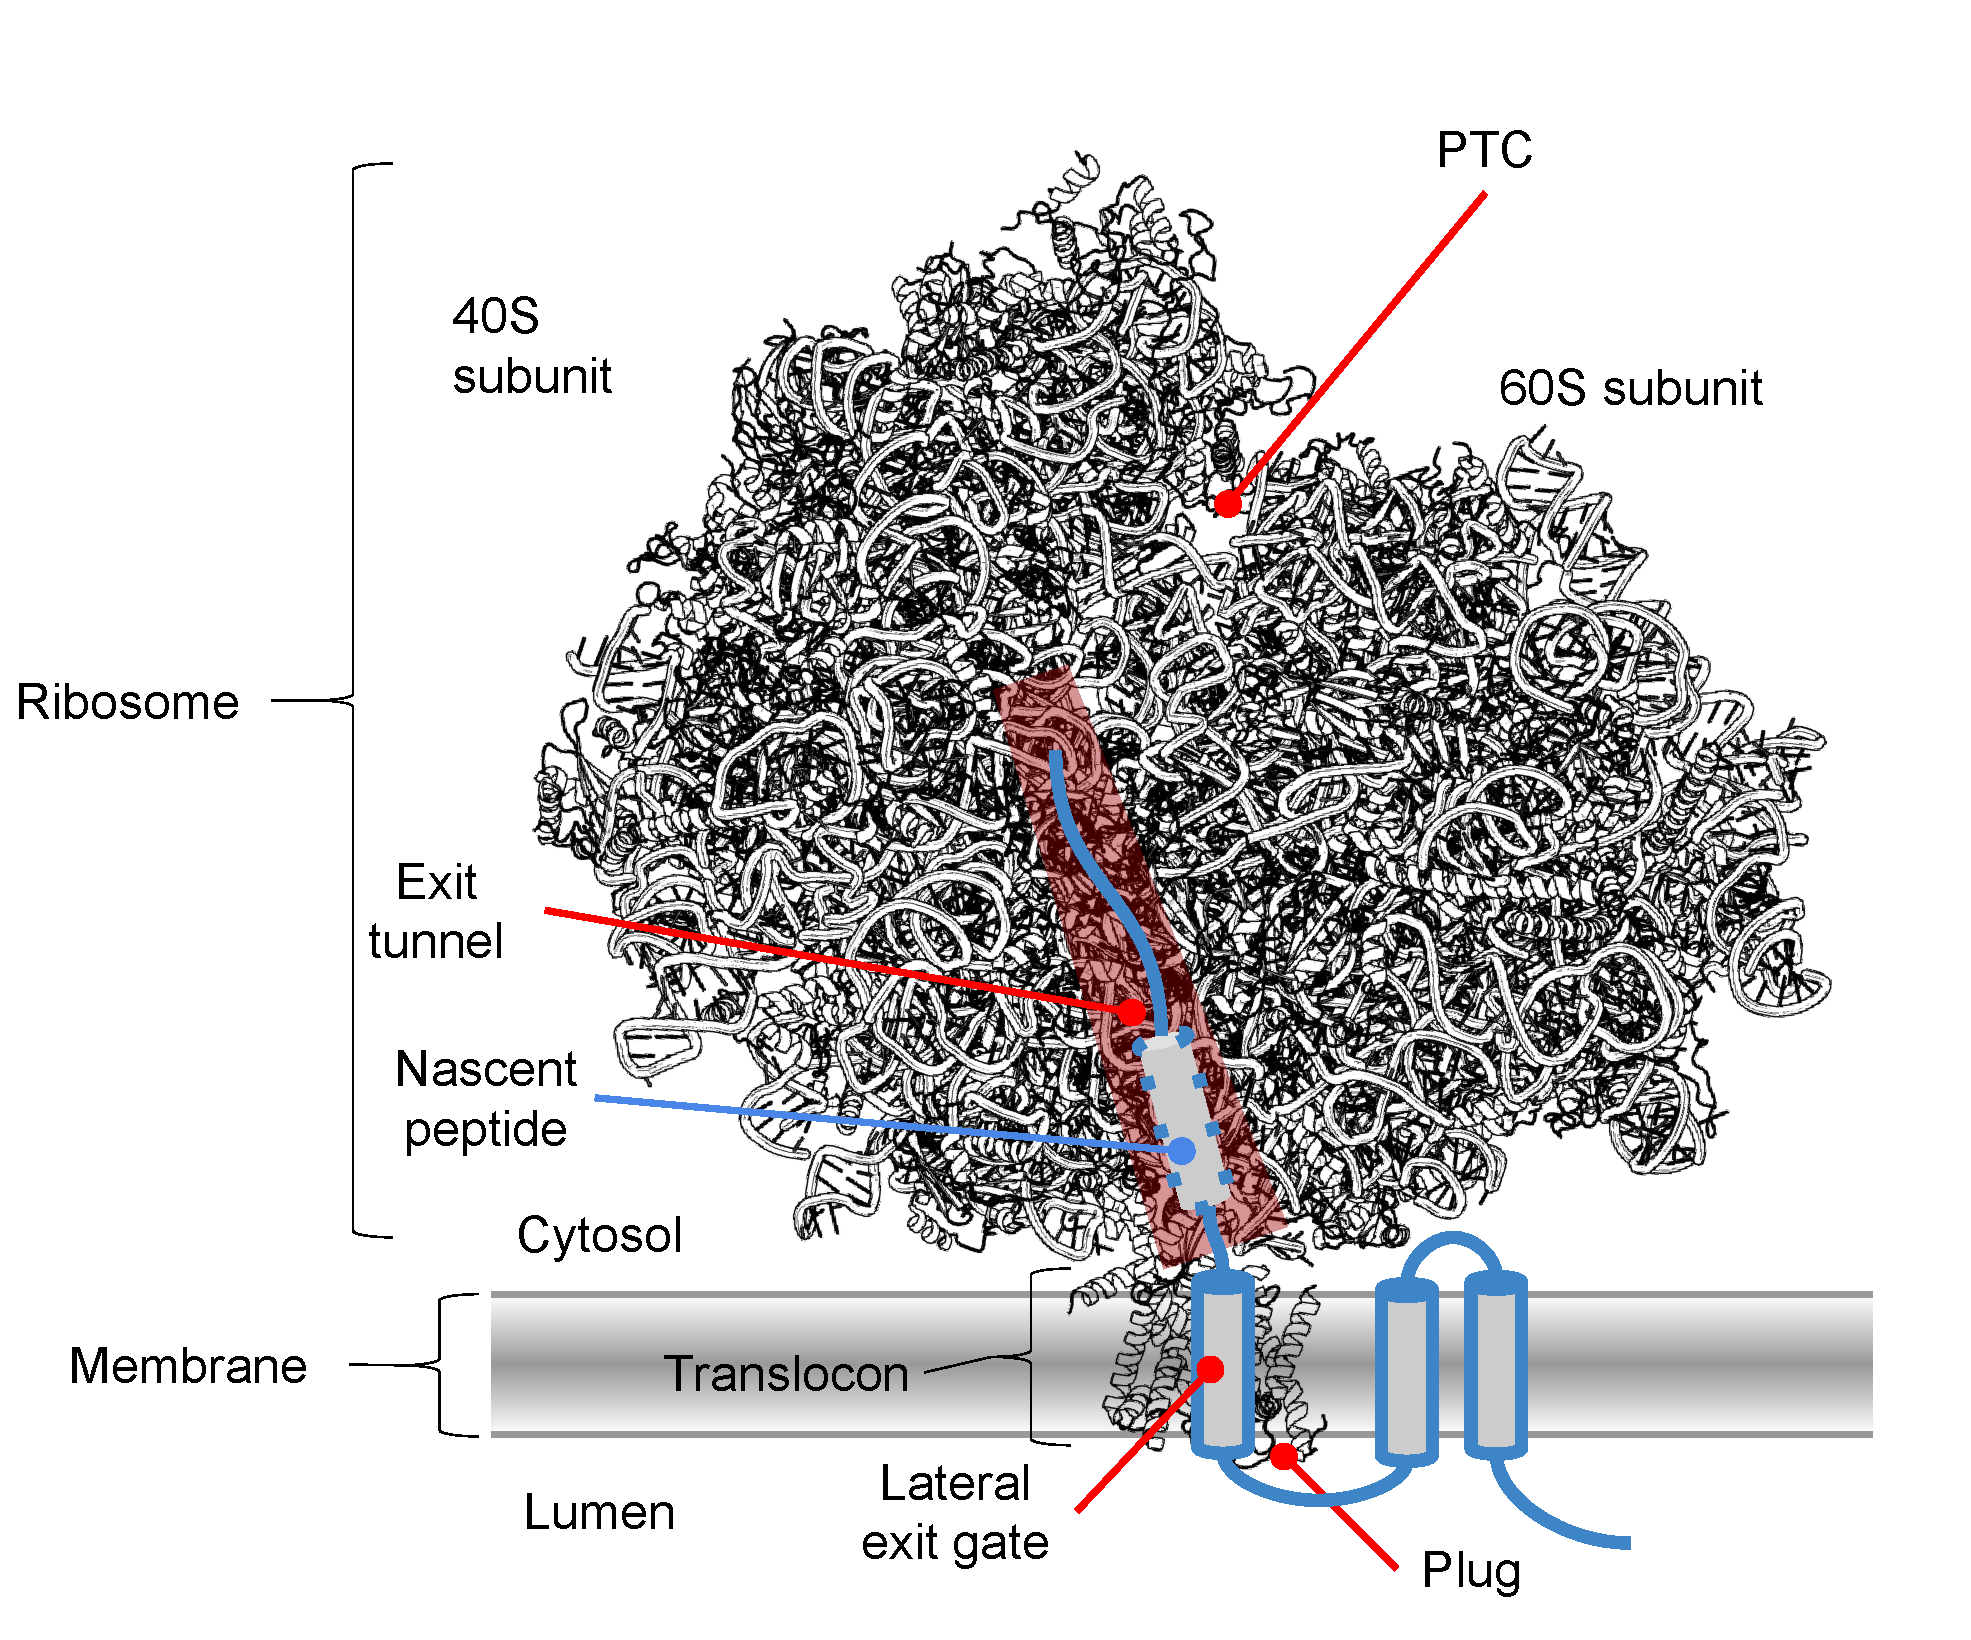
\includegraphics[width=1\textwidth]{multipass-folding/Ribosome-translocon-complex}
        \captionof{figure}[A cartoon of the ribosome in association with the translocon during insertion.]{\textbf{A cartoon of the ribosome in association with the translocon during insertion.}
        The structure used is of a translating mammalian ribosome-Sec61 translocon complex (PDB code 3j7r \cite{Voorhees2014}).
        The Sec61 translocon is the membrane\--embedded element of the structure that feeds the protein into the membrane.
        The ribosome is made of two elements; 60s and 40s.
        These vary in composition and size between eukaryotes and prokaryotes.
        PTC refers to the peptidase transferase centre, a high conserved catalytic site across all the kingdoms of life that performs the translation of \gls{rna} to amino acid polypeptides.
        After translation, the nascent peptide moves down the exit tunnel located in the larger ribosomal subunit (a simplified version of this channel is highlighted in red).
        There is evidence that the secondary structural elements of  \gls{tmh}s in ion channels are pre\--folded in the ribosomal exit tunnel \cite{Lu2005, Tu2010a, Tu2014, Kudva2018}.
        The ribosome hands the nascent chain to the translocon.
        Once the plug moves to expose the translocon pore, the translocon has a hydrophobic core which regulates the integration of the \gls{tmh} via the lateral gate \cite{Junne2010}.
}
\label{fig:Ribosome-translocon-complex}
\end{figure}

\gls{ap}s are typically 10-15 residues long that bind to the upper end of the ribosomal exit tunnel.
Once a specific mRNA codon is recognised, ribosomal stalling is induced \cite{Ito2010} and the translation is halted unless a strong enough pulling force from the downstream insertion is acting on the nascent chain at that time \cite{Butkus2003}.
Several ``strengths'' of \gls{ap} have been identified.
For example, SecM from \textit{E. coli} is 17 residues long and relatively weak, whereas a mutated SecM from \textit{Mannheimia succiniciproducens} (Ms-Sup1) is much stronger and 8 residues long ending in a proline which will halt translation \cite{Ismail2012}.
There are several other SecM proteins of other strengths from various bacterial species \cite{Yap2009}.
Therefore \gls{ap}s are a technique that can be used to measure precise forces acting on a specific part of the nascent chain during co-translational membrane protein integration allowing the study of \gls{tmp} kinetics during insertion and folding.
Indeed the force profile of a single residue can now be obtained \textit{in vivo} \cite{Ismail2012}.
In an idealised \gls{tmh} segment composed of alanine and leucine being inserted into \textit{E. coli} membrane through SecM \gls{ap} with SDS-PAGE, hydrophobicity is more able to overcome the arrest peptide when it is near the N\--terminal (of an N\--terminal-inside \gls{tmh}) \cite{Ismail2012}.
This could be either the \gls{tmh} finally coming into contact with the cytoplasmic face of the lipid bilayer, or an interaction between the N\--terminal and the tip of the lateral gate as previously shown in Sec61; part of a pre-integration \gls{tmh} interrogation \cite{MacKinnon2014}.

The ribosome passes the nascent chain to the Sec translocon machinery.
Like the ribosome, the Sec pathway is widely conserved across life \cite{Cao2003}.
Sec61 (in eukaryotes) and SecYEG (in prokaryotes) translocate hydrophilic peptides across a membrane whilst also integrating sufficiently hydrophobic sequences to the membrane~\cite{Junne2010, Park2012, Shao2011, Cymer2015}.
SecY in prokaryotes or Sec61$\alpha$ in eukaryotes are \gls{tmp}s with 10 \gls{tmh}s that perform the translocation.
These proteins have a lumenal plug~\cite{Tam2005, Junne2006} and a constricted core to prevent permeability whilst the protein is idle~\cite{Junne2010}.
During translocation the plug moves out of the pore \cite{Li2016}, the channel is in an open unconstricted state \cite{Junne2010}, and a lateral gate of TMH2 and TMH7 \cite{VandenBerg2004} periodically opens to release a \gls{tmh} to the membrane environment if sufficient hydrophobicity is present in the nascent peptide chain \cite{Niesen2018, Junne2010, Egea2010}(Figure \ref{fig:sequential-insertion}).


\subsection{Cooperative transmembrane helix insertion by the translocon-ribosome complex.}

Early evidence of secondary structure folding of the $K_{v}$ ion channel showed that the S6 \gls{tmh} (referred to later in this study as TMH6) is indeed compacted in the ribosomal tunnel by using pegylation and calmodulation of the tagged cysteine-scanned S6 transmembrane segment \cite{Lu2005}.
Furthermore, accessibility assays and an improved intramolecular  cross\--linking assay showed that the helical transmembrane S3\--S4 hairpin (the “paddle”) of a voltage-gated potassium ($K_{v}$) forms in the ribosome tunnel \cite{Tu2014}.
Ribosomal folding of the \gls{tmh}s in $K_{v}$1.3, a potassium channel, is maintained in the translocon \cite{Tu2010a}.
Therefore, some of the final structural folding of the voltage sensor domain occur within the ribosomal exit tunnel.

Furthermore, it has recently been suggested that larger structures fold as the ribosomal exit tunnel widens \cite{Kudva2018}.
This size\--dependent folding was observed by using the SecM translational \gls{ap}.
Two ribosome mutants of deleted uL23 and a uL24 variant that does not contain the hairpin loop were compared to the wild\--type (uL23 is a globular domain buried within the ribosome that is close to the exit tunnel and uL24 contains a hairpin loop that obstructs the tunnel exit).
These mutants resulted in reduced space for folding in the ribosomal exit tunnel at separate points.
ADR1a, a 29\-- residue zinc finger motif, was found to fold deeper in uL23 mutant than the wildtype and the uL24.
Two domain folds of 109 and 89 residues in length folded deeper in the uL24 mutant than in the wild\--type and the uL23 mutant.
This shows that  cotranslational folding can occur in the ribosomal exit tunnel once sufficient space is available \cite{Kudva2018}.

The ribosomal tunnel also speeds up elongation of neutral and negatively-charged peptides.
This is attributed to the sporadic negative patches within the ribosomal exit tunnel \cite{Lu2008}.

The ribosome clearly has the potential to pre\--fold secondary structures and some motifs before translocon insertion into the membrane.

Multiple \gls{tmh}s in a nascent protein can be associated with the eukaryotic translocon simultaneously.
It was shown that \gls{tmh}s can stay in association with the translocon in order to mediate integration of downstream \gls{tmh}s demonstrated by  cross\--linking analysis \cite{Sadlish2005, Cross2009}.
Not only this, but it was shown that there is a direct interaction between the \gls{tmh}s; more recently \gls{ap}s were used to show pulling forces between a \gls{tmh} and more C-terminally located \gls{tmh} during the C-terminal \gls{tmh} membrane partitioning from the translocon \textit{in vivo} \cite{Cymer2013}.
This could be facilitated during the probing of a \gls{tmh} from the translocon as the lateral gate ``cracks'' open in an intermediate stage before the \gls{tmh} satisfies the full hydrophobic requirements to open the gate fully, an intermediate stage observed in a SecY crystal structure \cite{Egea2010}.

Sixteen marginally hydrophobic \gls{tmh}s were screened and revealed that independently they did not efficiently insert via the translocon into the \gls{er} \cite{Hedin2010}.
The study showed that in the presence of the neighbouring loops and \gls{tmh}s, insertion often became sufficient with the exception of two of the marginally hydrophobic \gls{tmh}s.
The orientational preference of neighbouring \gls{tmh}s was shown to increase insertion efficiency into the \gls{er} of a marginally hydrophobic \gls{tmh} \cite{Ojemalm2012}.
A glycosylation study of three relatively polar \gls{tmh}s revealed that proteins have even evolved to exhibit stronger ``positive\--inside'' tendencies when following another \gls{tmh} \cite{Virkki2014}.
Subsequent \gls{tmh}s with a strong topological preference (increased arginine presence) increase the insertion potential of relatively polar \gls{tmh}s, however, no specific interaction between the \gls{tmh}s was responsible.
The nascent polypeptide in the cavity between the ribosome and the translocon can
alter the hydrophobic threshold of the translocon is dynamic and influenced by downstream flexible sequences \cite{Junne2017}.
Sequence context is clearly an important factor of the efficient insertion of marginally hydrophobic \gls{tmh}s; these \gls{tmh}s rely on other components of their protein in order to incorporate into the membrane.

\section{Methods}
\subsection{Datasets}
\subsubsection{Membrane protein families}
This is not an exhaustive search among \gls{tmp}s for all examples of starkly polar \gls{tmh}s conserved among the family.
Instead, we show that there is a precedent for several, but not all, protein families to contain polar helices and that these polar \gls{tmh}s are sequentially next to typically hydrophobic \gls{tmh}s.
Analysis can only be done if the number of \gls{tmh}s is conserved across the family since different mechanisms are utilised to transmit a signal or transport a molecule across the membrane.

Datasets were attained by querying the UniProt database for controlled vocabulary keywords (Table \ref{table:datasetsizes}) \cite{TheUniProtConsortium2014}.
After filtering out redundant proteins using UniRef50, the datasets were stratified according to the total number of \gls{tmh}s per protein.
Only families with a total N \textgreater 20 were included in the analysis, for example, there are ion channels with 12 \gls{tmh}s, but only 16 examples fitted the criteria and were omitted from the study.



\begin{table}[htbp]

  \centering
  \captionof{table}[Dataset sizes of common transmembrane protein families of transporters and channels.]{\textbf{Dataset sizes of common transmembrane protein families of transporters and channels.}
  The type column refers to the family name.
  The keyword identifier column refers to the specific query term that UniProt uses as the controlled vocabulary identifier.
  UniProt hits refers to the number of SwissProt hits, which are manually curated, however, the SwissProt and TrEMBL hits are also given in the brackets.
  The UniRef column denotes how many representative sequences resulted from the UniProt hits, again with the number in the brackets including the TrEMBL hits.
  Because UniRef often returns representatives of splice isoforms as a separate hit, the lists were re-uploaded to UniProtKB to get the final hit.
  The lists are then stratified by the total number of TMHs.
  }
\footnotesize
\begin{tabular}{lllllll}

  Type                     & KW & UniProt Hits   & UniRef &  Records & TMHs & Final hits \\
  Ion channel              & 0407            & 2452 (176417)  & 912 (21024)            & 882                & 4    & 234        \\
                           &                    &                &                        &                    & 6    & 188        \\
                           &                    &                &                        &                    & 24   & 34         \\
  Ligand\--gated ion channel & 1071            & 452 (14051)    & 189 (3055)             & 185                & 6    & 33         \\
  Voltage\--gated channel    & 0851            & 683 (27,662)   & 285 (3876)             & 267                & 6    & 97         \\
  Calcium channel          & 0107            & 272 (5056)     & 128 (1003)             & 120                & 6    & 38         \\
  Potassium channel        & 0631            & 337 (11852)    & 160 (1893)             & 152                & 6    & 88         \\
  Sugar transport          & 0762            & 1217 (107721)  & 467 (16748)            & 464                & 12   & 134        \\
  Chloride channel         & 0869            & 303 (3697)     & 117 (1039)             & 117                & 4    & 50         \\
  Ion transport            & 0406            & 10264 (443600) & 3070 (42259)           & 3023               & 4    & 338        \\
                           &                    &                &                        &                    & 6    & 390        \\
                           &                    &                &                        &                    & 8    & 162        \\
                           &                    &                &                        &                    & 10   & 189        \\
                           &                    &                &                        &                    & 12   & 292        \\
                           &                    &                &                        &                    & 24   & 35
\end{tabular}
\label{table:datasetsizes}
\end{table}


\subsubsection{GPCR subfamilies}
The 7TMR list is a list distributed by UniProt containing \gls{gpcr}s available at \url{http://www.uniprot.org/docs/7tmrlist.txt} \cite{TheUniProtConsortium2014}.
The entire list contains 3115 UniProt IDs which mapped to 3092 records on the date of download (12/9/2017).
After removing redundant records using UniRef50 to identify cluster representatives, 1142 records made the final dataset.
The original list is also sub categorised by function.
Here, we also looked at opsins, the T2R taste receptors, frizzled/smooth \gls{gpcr}s, metabotropic glutamate receptors (Family C), and fungal mating proteins.

218 opsin records were mapped through UniRef50 to 40 records.
211 T2R taste receptors were mapped to 45 records after UniRef50.
There were 82 records for frizzled/smooth, of which 41 were cluster representatives after querying with UniRef50.
114 were metabotropic glutamate receptors which became 44 after redundancy removal.
In serotonin, 91 original records were represented by 28 records.
There were 13 fungal mating proteins, represented by 9 after UniRef50.
560 olfactory records were mapped to 274 records after Uniref50.

After limiting all these sets to records containing 7 TRANSMEM features, there were 39 opsins, 38 frizzled smooth \gls{gpcr}s, 9 fungal mating \gls{gpcr}s, 41 metabolic glutamate receptors, 45 t2r taste receptor proteins, and 263 olfactory receptor \gls{gpcr} proteins.
TRANSMEM is an annotation by UniProt denoting a \gls{tmh} evidenced by experimental documentation or a robust \gls{tmh} prediction method \cite{TheUniProtConsortium2014}.


\subsection{Gene ontology}
77153 protein records matched the query \url{annotation:(type:transmem) AND reviewed:yes} in UniProt \cite{TheUniProtConsortium2014}.
30045 records of these represented those proteins after submitting the list to UniRef50.
To gain an approximate idea of what proteins may have cooperative \gls{tmh}s, we submitted that non-redundant SwissProt transmembrane dataset to PANTHER and used their pie chart visualisation \cite{Mi2017}.
We also submitted a constricted list of the non-redundant SwissProt transmembrane dataset to PANTHER by sorting the list according to proteins with sequentially adjacent \gls{tmh}s that had the greatest difference in Kyte \& Doolittle hydrophobicity \cite{Kyte1982}.
This consisted of the top 102 pairs from a list of 101604 (the top 0.1\%) \gls{tmh} pairs from 87 unique UniProt records.
In PANTHER, these hit 59 genes with 58 functions.

\subsection{Complexity and hydrophobic estimation}
Primarily we used the Kyte \& Doolittle scale in this work \cite{Kyte1982}.
We verified this scale with the Eisenberg scale \cite{Eisenberg1984}, the Hessa biological scale \cite{Hessa2005}, and the White and Wimley scale \cite{White1999}.
The Eisenberg scale is potentially double counted for many of these proteins since it is used by UniProt during their automatic \gls{tmh} annotation where experimental evidence is not available.
The Hessa biological scale originally reported positional dependencies that affected the hydrophobicity values which were refined in a later version of the scale \cite{Hessa2007}, however, this later version was not programmatically available to us.

When stratifying \gls{tmh}s by hydrophobicity and sequence information entropy, there is a clear distinction between anchoring \gls{tmh}s and those with a function beyond anchoring.
The TMSOC  z\--score quantifies this relationship and is calculated by equation \ref{equation:zscoreterm2}.

\begin{equation} \label{equation:zscoreterm2}
z({x}_{\Phi},{x}_{c})={(-1)}^{s}\left[\frac{{({x}_{\Phi}-{\mu}_{\Phi})}^{2}}{{\sigma}_{\phi}^{2}}+\frac{{({x}_{c}-{\mu}_{c})}^{2}}{{\sigma}_{c}^{2}}\right]
\end{equation}

$x_c$ and $x_\Phi$ are moving window averages of c, the sequence entropy~\cite{Wootton1996}. $\Phi$ is the White and Wimley hydrophobicity~\cite{White1999} for a given segment and $\mu$ and $\sigma$ are the mean and standard deviation of the sequence entropy and hydrophobicity of the functional~\gls{tmh} sets.

\subsection{Statistics}

We used the Welch's t\--test to scrutinise the means of the datasets without assuming equal variance.
To examine any differences in the skew of the datasets, the Kruskal Wallis, and the Kolmogorov Smirnov tests were used.
All these tests were performed using the Python scipy package \cite{Oliphant2007}.


\section{Results and discussion}

\subsection{Large contrasts in transmembrane helix hydrophobicity occur in channels and receptors.}
Large differences in sequenctially adjacent \gls{tmh}s could indicate cooperative insertion mechanisms of marginally hydrophobic \gls{tmh}s.
In order to identify which type of \gls{tmp} may contain cooperative \gls{tmh}s, the hydrophobicities for \gls{tmh}s from 30045 records in a non-redundant version of SwissProt were calculated according to the Kyte \& Dolittle hydropathy scale \cite{Kyte1982}.
The absolute difference between each sequentially adjacent \gls{tmh} was calculated.
The full list, along with the 0.1\% \gls{tmh} pair were submitted to PANTHER \cite{Mi2017}.
We found that transporters were by far the most abundant in this sub\--list relative to the global TMP list, however, it should be considered that ``transporters'' in this sense also includes both ion transporters and ion channels (Figure \ref{fig:good-bad-ontology}).
Among the other prevalent functions are receptors, binding proteins, and signal transducers.
All these lists were predominantly made up of \gls{gpcr}s.


\begin{figure}[!ht]
\centering
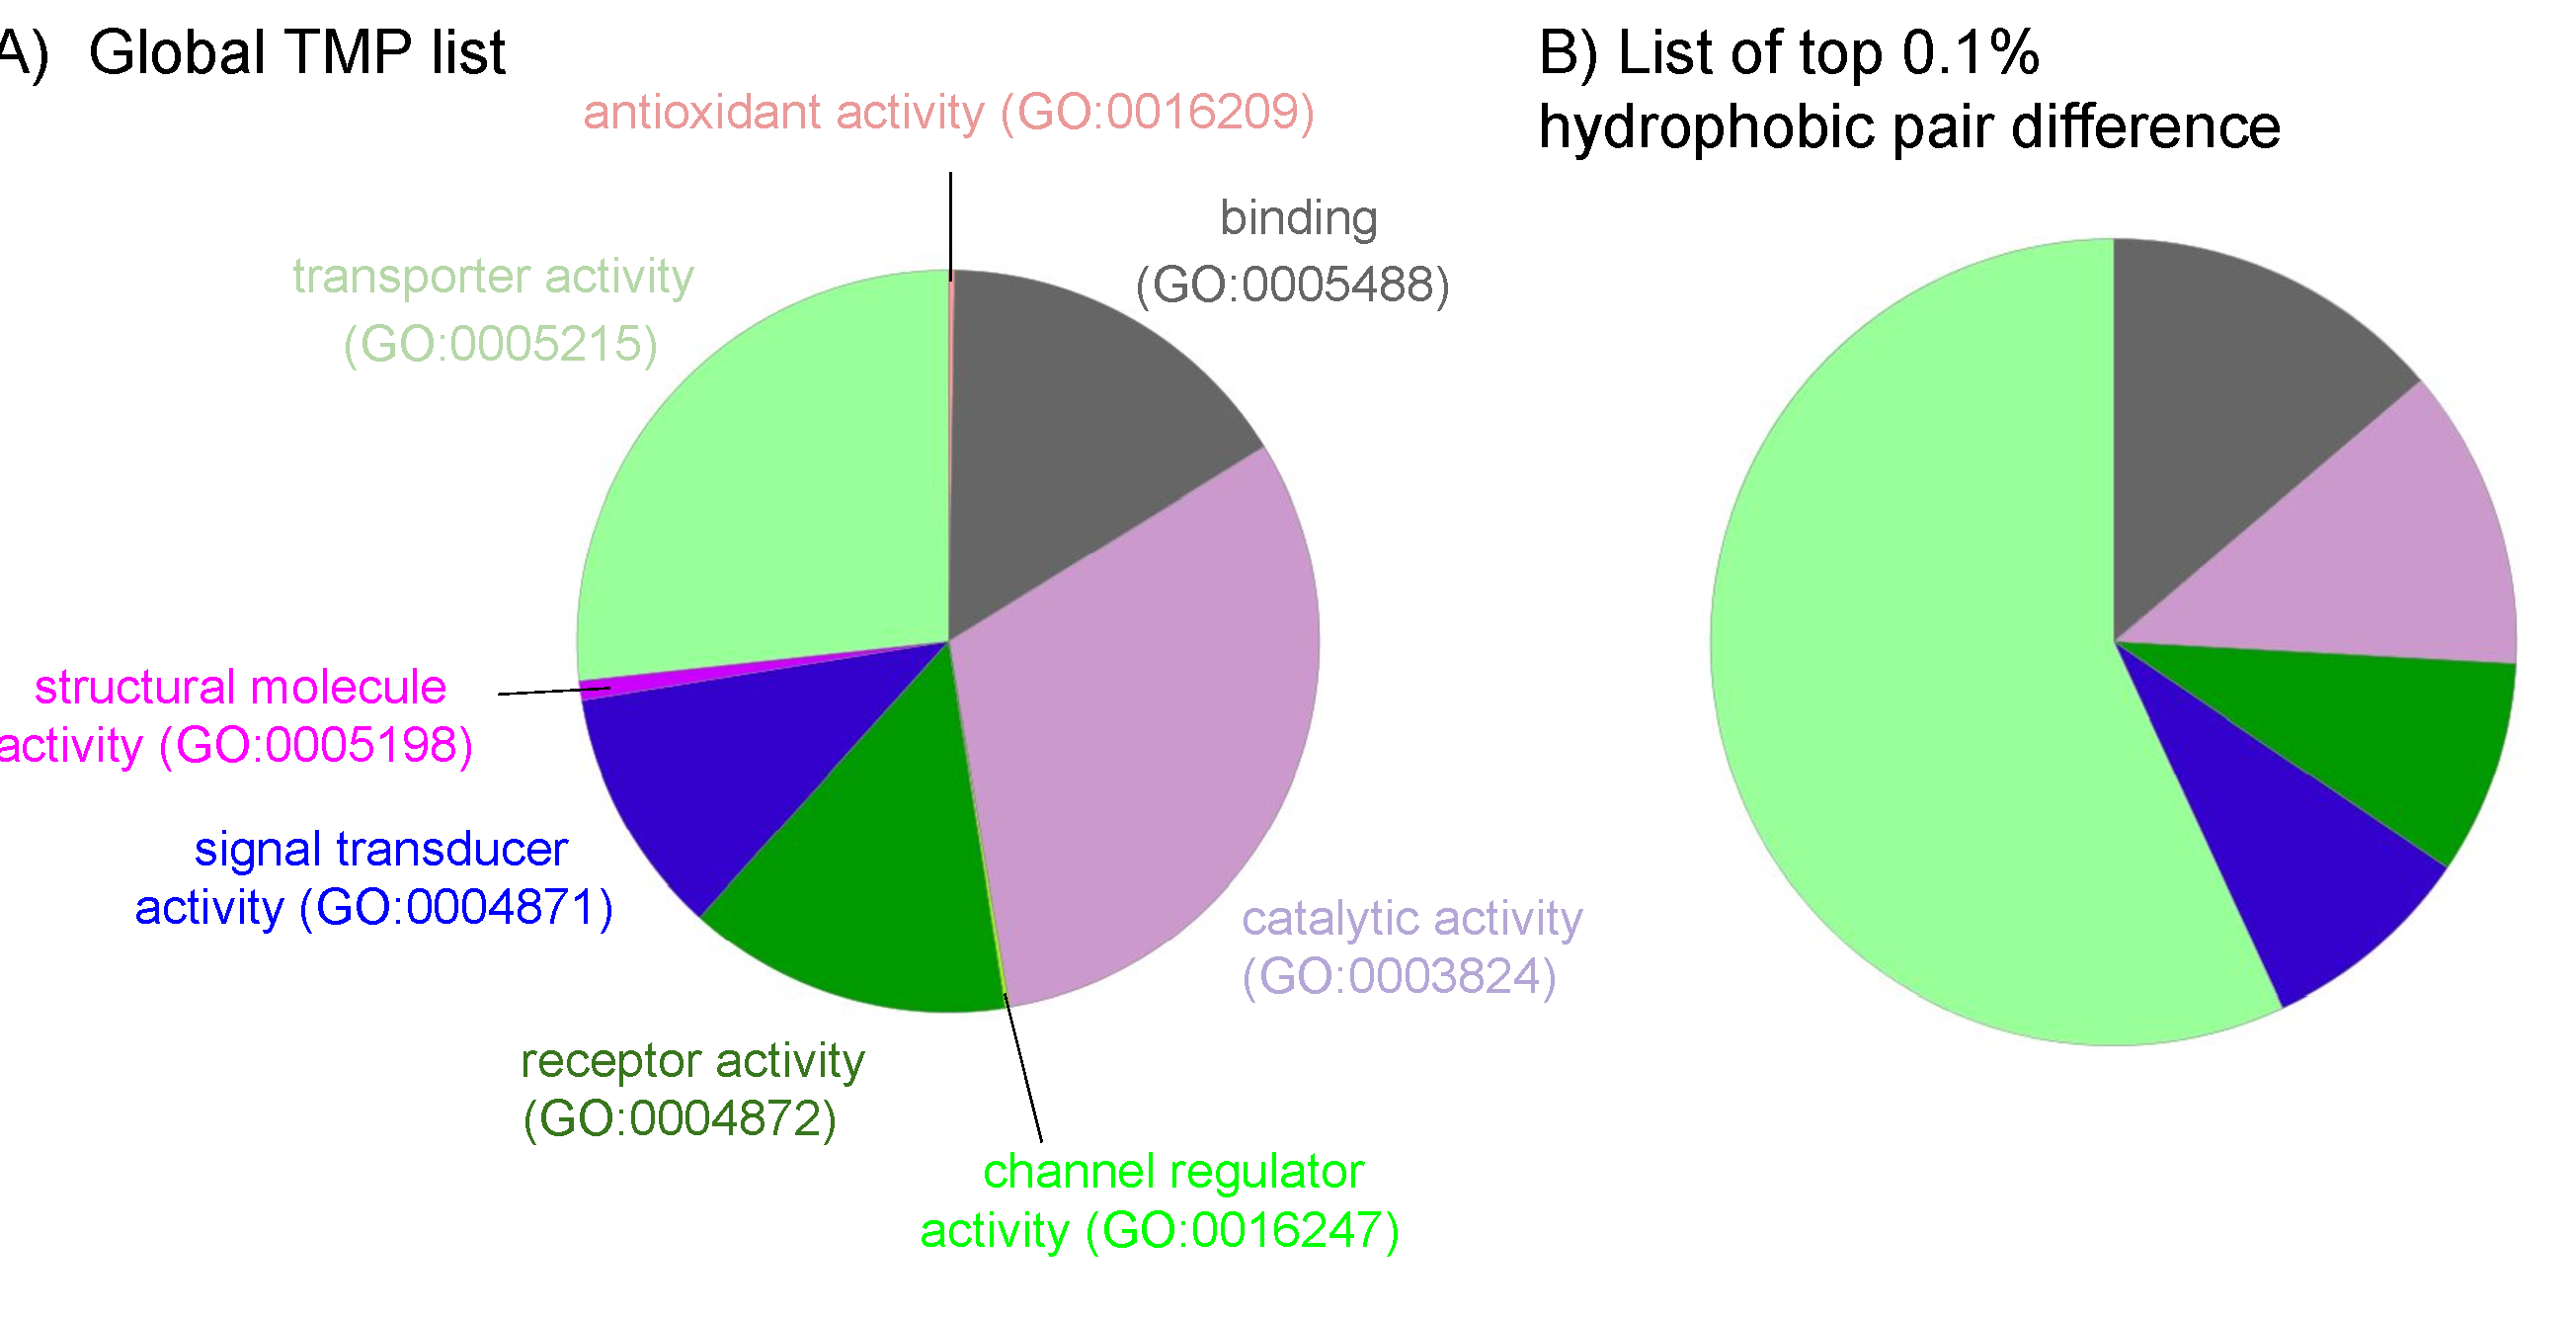
\includegraphics[width=1\textwidth]{multipass-folding/good-bad-ontology}
		\captionof{figure}[Pie charts of a non-redundant list of transmembrane proteins compared to a list of transmembrane proteins containing the most hydrophobically different transmembrane helix pairs.]{\textbf{Pie charts of a non-redundant list of transmembrane proteins compared to a list of transmembrane proteins containing the most hydrophobically different transmembrane helix pairs.}
    The output of PANTHER Gene ontology server of A) a non-redundant list of all TMPs in SwissProt and
    B) a list of the TMPs with the highest (0.1\%) hydrophobic discrepancy between adjacent TMHs.
    Note that the proportions of binding TMPs stay roughly the same, receptors and signal transducers reduce slightly, catalytic proteins are reduced by two thirds and transporter more than doubles in proportion.
    }

\label{fig:good-bad-ontology}
\end{figure}

Since catalytic function decreased so much, as a trend we thought that the catalytic function of the \gls{tmp} may not be associated with a high hydrophobic discrepancy between \gls{tmh}s within the protein.
This gives us an idea of search space where highly polar \gls{tmh}s are proximally adjacent to typically hydrophobic \gls{tmh}s; \gls{gpcr}s and membrane transporters.
%Need percentage decreases

\subsection{GPCRs contain conserved relatively polar TMH7, which follows the typically hydrophobic TMH6}

\gls{gpcr}s are a diverse family of membrane surface receptors with 7 \gls{tmh} segments.
GPCRs have long been known to be overrepresented among genomes \cite{Remm2000}.
They have adapted to respond to a wide range of specific signals ranging from macromolecules to photons.
The specific signal triggers a conformational change of the \gls{gpcr} that is translated across the membrane.
\gls{gpcr}s have been associated with tumorigenesis \cite{OHayre2013}, metastasis \cite{Singh2015} and in cancers \cite{Bar-Shavit2016} and are a potential target for therapies \cite{Arakaki2018}.
Their ubiquitous presence in cellular life and medical relevance makes them an important topic of study.

Here, we structurally aligned 7 structures of monomeric \gls{gpcr}s using PyMol \cite{DeLano2002};
PDB codes 1u19 (rhodopsin) \cite{Okada2004}, 2z73 (rhodopsin) \cite{Murakami2008}, 2vt4 ($\beta$1-adrenergic receptor) \cite{Warne2008}, 2lnl (CXCR1, rhodopsin-like) \cite{Park2012}, 4mbs (CCR5, chemokine receptor) \cite{Tan2013}, 4xt1 (viral chemokine) \cite{Burg2015}, and 4ea3 (opioid receptor) \cite{Thompson2012} (Figure \ref{fig:GPCR-structures}A).

\begin{figure}[!ht]
\centering
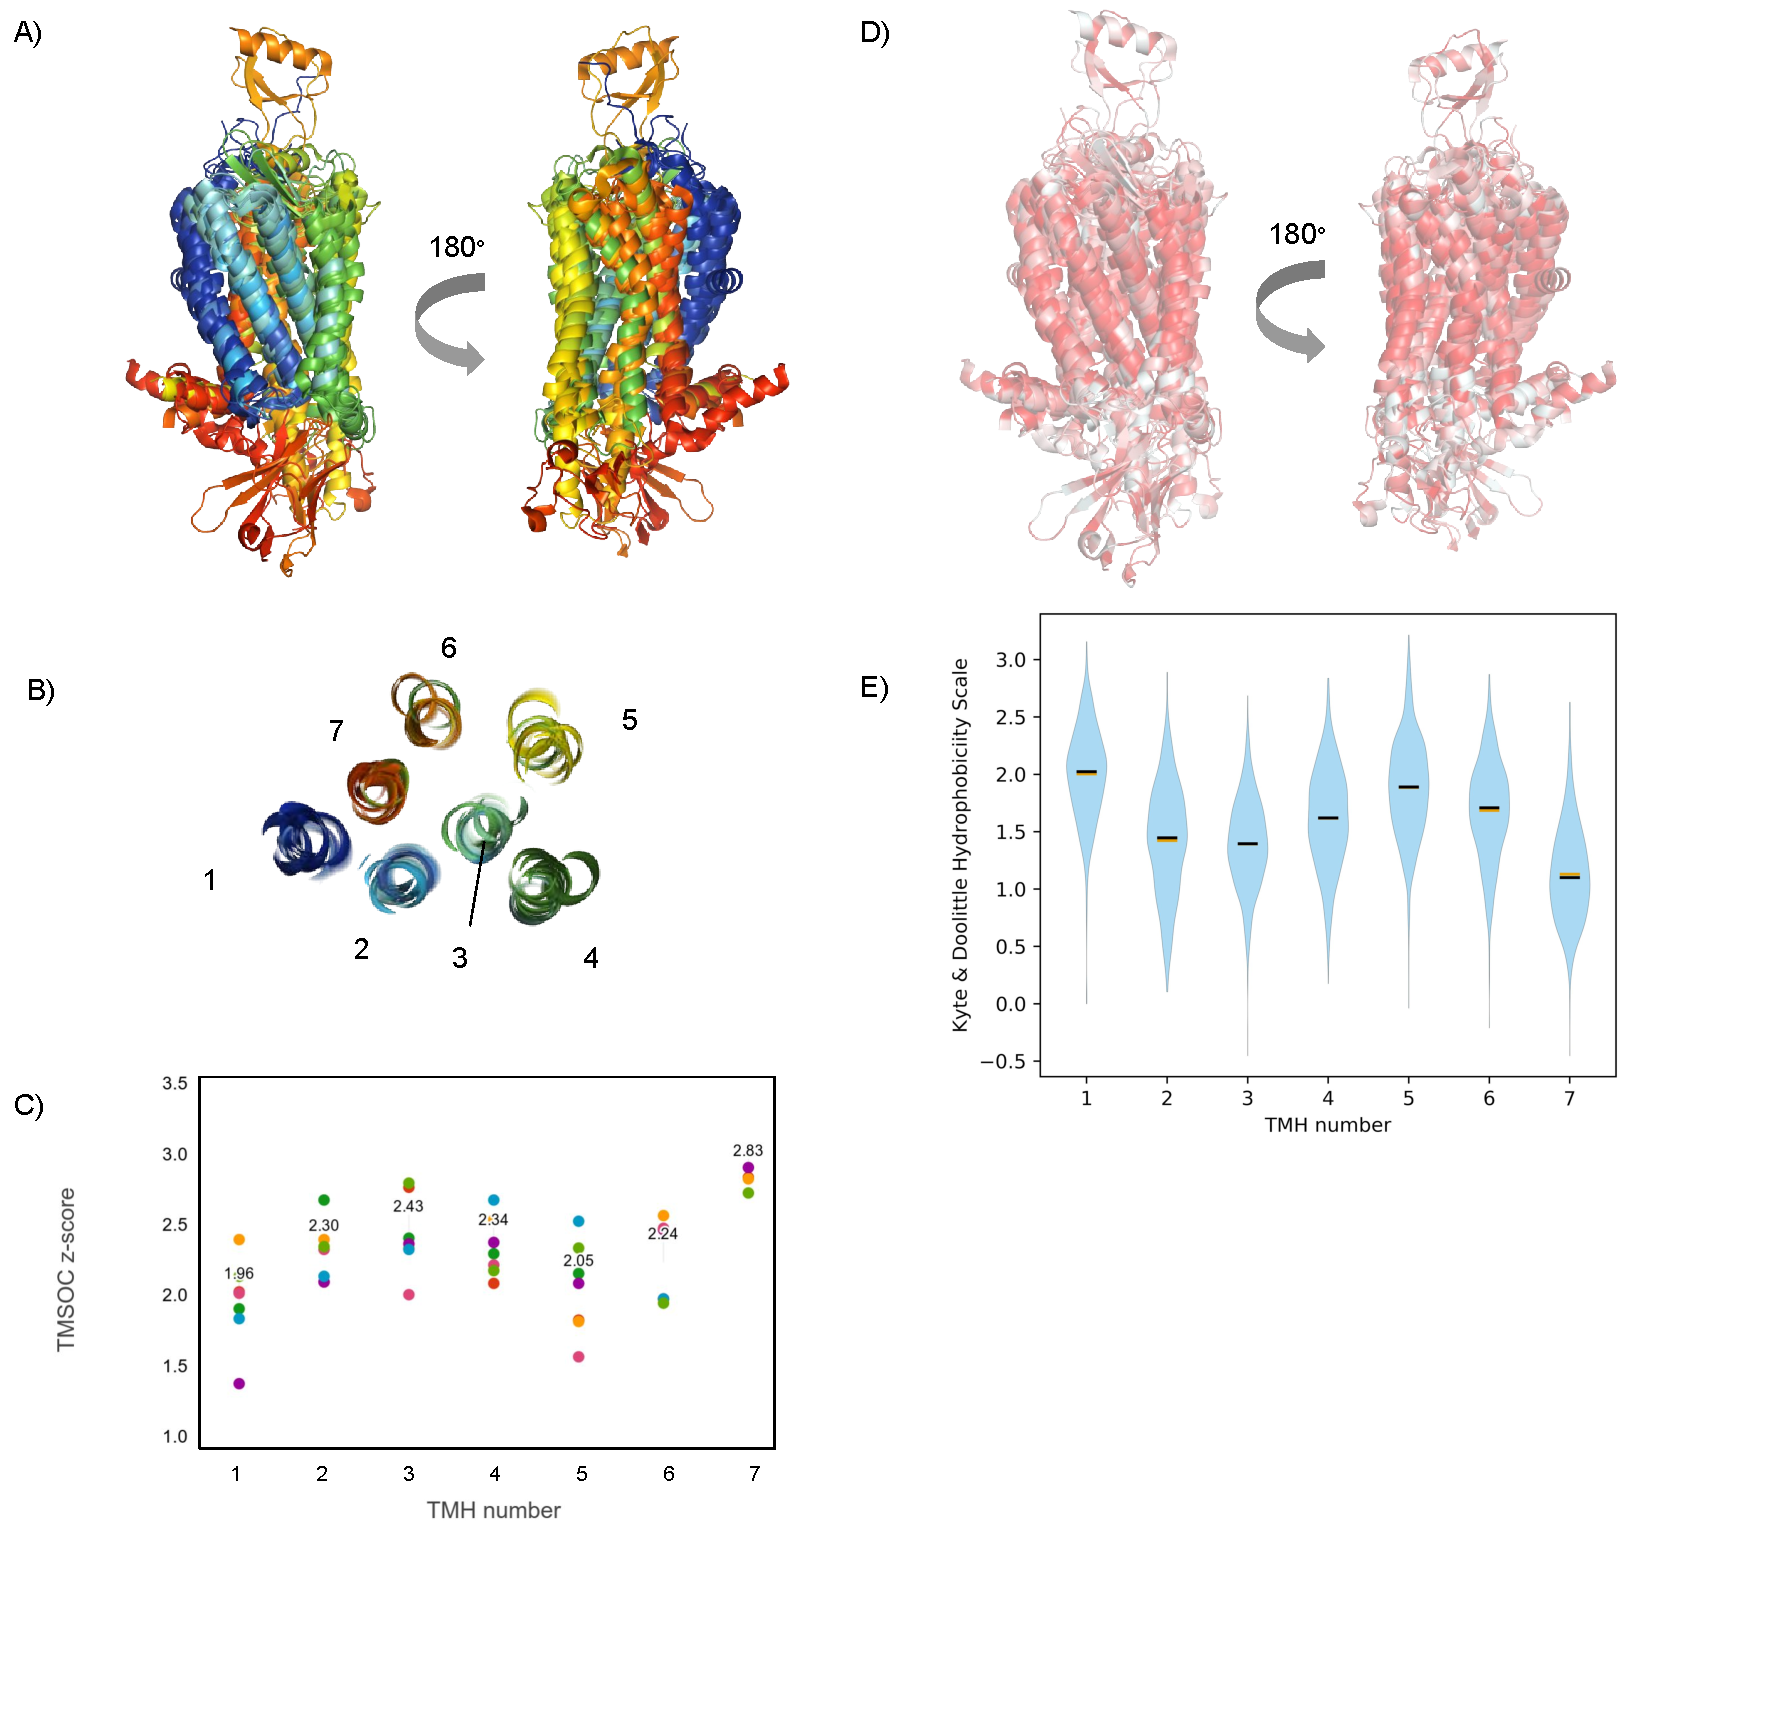
\includegraphics[width=1\textwidth]{multipass-folding/GPCR-structures}
		\captionof{figure}[The hydrophobicity and complexity of GPCR transmembrane helices.]{\textbf{The hydrophobicity and complexity of GPCR transmembrane helices.}
    A) A cartoon of 7 structurally aligned \gls{gpcr}s of various molecular functions coloured according to the residue sequence position.
    Blue is the N terminal residue, working through the rainbow until red at the C terminal position.
    B) The same 7 \gls{gpcr}s aligned structurally but instead coloured by the Eisenberg hydrophobic scale \cite{Eisenberg1984} at 50\% transparency with red being hydrophobic and white being polar.
    C) A top\--down (birds\--eye) version of the alignment coloured similarly to A taken at a slice halfway through the TMHs.
    D) On the vertical axis is the TMSOC z\--score of each of the helices and on the horizontal axis is the TMH number.
    The points are coloured by the corresponding structure.
    E) The axes are similar to D, however, the datasets are from non-redundant UniProt \gls{gpcr} sequence datasets from 1016 \gls{gpcr} records that contained the annotation for 7 \gls{tmh}s.
    The data is represented by a violin plot, the thickness indicating the distribution of the data.
    The mean average is the dash in black, and the median is the dash in orange.
    F) As in E, however, the vertical axis is Kyte \& Doolittle hydrophobicity \cite{Kyte1982}.}

\label{fig:GPCR-structures}
\end{figure}

Even in a relatively small dataset of functionally varied \gls{gpcr}s, we can see structural conservation of the \gls{tmh} arrangement (Figure \ref{fig:GPCR-structures}A Figure \ref{fig:GPCR-structures}C).
Hydrophobic patterns are hard to identify structurally beyond the clear membrane boundary where we would expect to see hydrophobic residues in the \gls{tmh} (Figure \ref{fig:GPCR-structures}B).
TMSOC \cite{Wong2011, Wong2012} is an algorithm that takes into account the White and Wimley hydrophobicity \cite{White1999} and the information entropy of the TMH sequence.
Note that the scale is the inverse of the Kyte \& Doolittle scale, i.e a more negative score indicates a higher hydrophobic contribution in TMSOC z\--score, and a more positive value indicates higher hydrophobicity.
The resulting z\--score has been shown to be able to scrutinise between \gls{tmh}s that serve as anchors and those that have a function beyond \gls{tmp} anchoring.
The lower the z\--score (low sequence information entropy and high hydrophobicity), the more likelihood of the \gls{tmh} being solely a membrane anchor.
When considering the functional/anchoring potential of these \gls{gpcr} \gls{tmh}s  using TMSOC, we see trends among the structures with an average of 1.96 for TMH1, 2.30 for TMH2, 2.43 for TMH3, 2.34 for TMH4, 2.05 for TMH5, 2.24 for TMH 6 and 2.83 for TMH7 (Figure \ref{fig:GPCR-structures}D).
TMH3 and TMH7 are therefore the most likely to contain function beyond anchorage, whilst the low z\--scores of TMH1 and TMH5 indicate they are more optimal anchors \cite{Baker2017}.

When we consider much larger sequence datasets containing 1016 \gls{tmh}s at each \gls{tmh} number from non-redundant \gls{gpcr}s obtained from UniProt, the trend remains the same: that TMH3 (mean z\--score of 2.52) and TMH7 (mean z\--score of 2.55) have the highest z\--score, whilst TMH1 (mean z\--score of 2.09) and TMH5 (mean z\--score of 2.20) have the lowest (Figure \ref{fig:GPCR-structures}E).
To investigate the statistical differences between the z\--score of the \gls{tmh}s, we applied the Kruskal Wallis and 2-sample Kolmogorov Smirnov tests from each \gls{tmh} number to each other \gls{tmh} number.
TMH5 and TMH7 are statistically significantly distinct in terms of TMSOC z\--score (Welch's t-test P\--value = 1.57E\--146, Kruskal Wallis P\--value = 1.66E\--132, Kolmogorov Smirnov P\--value = 1.38E\--105) as are TMH6 and TMH7 (P\--value = 1.48E\--51, Kruskal Wallis P\--value = 4.96E\--52, Kolmogorov Smirnov P\--value = 1.74E\--37).
This is also mirrored in the relationship between the preceding \gls{tmh}s of TMH3.
TMH1 and TMH3 are distinct (Welch's t-test P\--value = 3.12E\--229, Kruskal Wallis P\--value = 1.06E\--192, Kolmogorov Smirnov P\--value = 1.06E\--174) and so are TMH2 and TMH3 (Welch's t-test P\--value = 3.66E\--39, Kruskal Wallis P\--value = 2.70E\--36, Kolmogorov Smirnov P\--value = 1.06E\--31).
We also find it difficult to observe any significant differences between TMH2 and TMH6 (Welch's t\--test P\--value \textgreater 0.99, Kruskal Wallis P\--value = 0.99, Kolmogorov Smirnov P\--value = 0.07).

As expected, these trends are mirrored in the Kyte \& Doolittle \cite{Kyte1982} hydrophobicity plots.
Where there is a high TMSOC z\--score, there is a low hydrophobicity score.
However, whereas TMH6 (mean hydrophobicity = 1.69) to TMH7 (mean hydrophobicity = 1.13) are very different (Welch's t\--test P\--value = 3.95E\--163), the difference between TMH2 (mean hydrophobicity = 1.42) and TMH3 (mean hydrophobicity = 1.39) is less stark (Welch's t\--test P\--value = 0.12).
Even though there is a discrepancy between the scales, the significant change in hydrophobicity  between TMH6 and TMH7 can be seen consistently across the Eisenberg consensus scale \cite{Eisenberg1984} (Welch's t\--test P\--value = 5.61E-130), the White and Wimley biophysical scale \cite{White1999} (Welch's t\--test P\--value = 5.21E-62), and the von Heijne/Hessa biological scale \cite{Hessa2005} (Welch's t\--test P\--value = 3.56E-210) emphasising the significance of this particular \gls{tmh} pair (Figure \ref{fig:gpcr-hydrophobicity-verification}).

\begin{figure}[!ht]
\centering
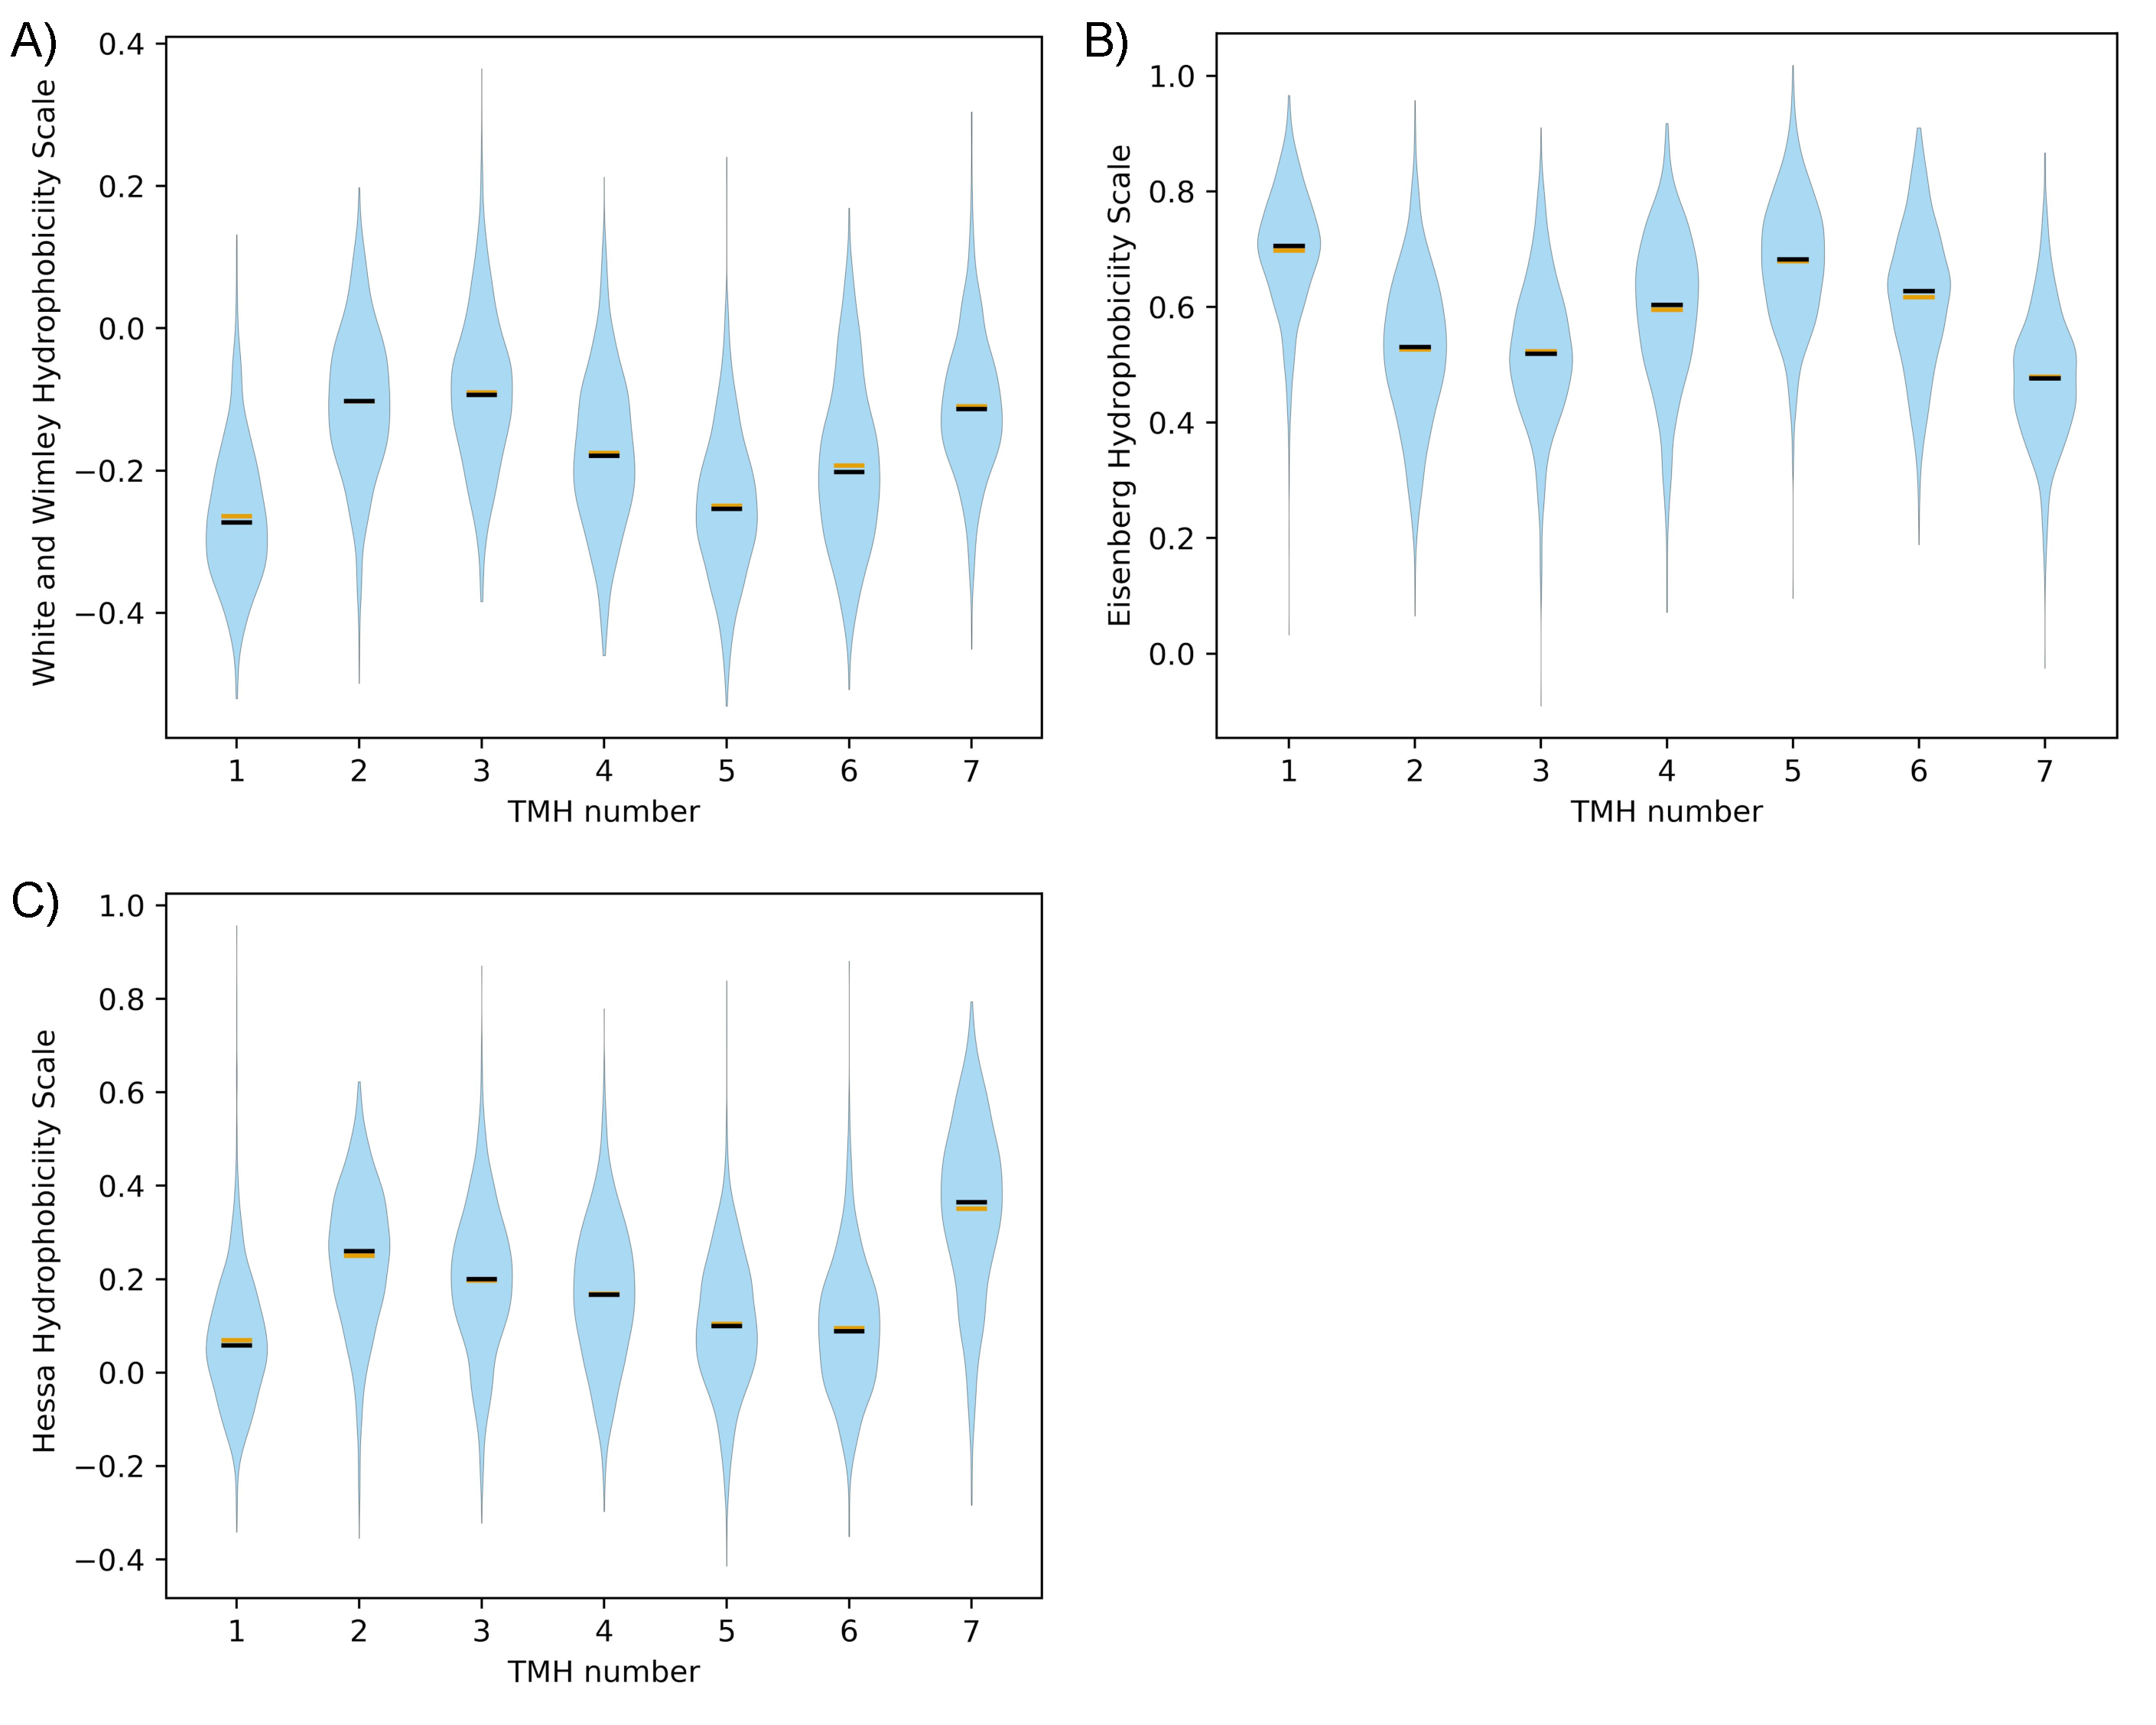
\includegraphics[width=1\textwidth]{multipass-folding/gpcr-hydrophobicity-verification}
		\captionof{figure}[The hydrophobic difference observed between TMH6 and TMH7 in GPCRs is not due to the choice of hydrophobic scale.]{\textbf{The hydrophobic difference observed between TMH6 and TMH7 in GPCRs is not due to the choice of hydrophobic scale.}
    Three different scales were applied to the same dataset used in figure \ref{fig:GPCR-structures}F to verify the observed differences were not caused by the choice of scale.
    A) The White and Wimley biophysical scale \cite{White1999}
    B) The Eisenberg consensus scale \cite{Eisenberg1984}.
    C) The von Heijne/Hessa biological scale \cite{Hessa2005}.}

\label{fig:gpcr-hydrophobicity-verification}
\end{figure}

In order to determine if this is conserved through the \gls{gpcr} subfamilies, a variety of \gls{gpcr}s with different functions were examined in terms of Kyte \& Doolittle hydrophobicity.
When considering different \gls{gpcr} subfamilies, we see a consistent difference between hydrophobicities between TMH6 and TMH7 besides metabolic glutamate \gls{gpcr}s (Welch's t\--test P\--value = 0.90) and Frizzled-smooth \gls{gpcr}s (Welch's t\--test P\--value = 0.07) in which there is only a little discrepancy (Figure \ref{fig:KD-GPCR}).
For opsins, Welch's t\--test P\--value is 5.62E-15.
After restricting the dataset to only those records with 7 \gls{tmh}s, fungal mating \gls{gpcr}s were reduced to a set of 9 proteins, however as a trend, they appear to be very typical \gls{gpcr}s in terms of \gls{tmh} hydrophobicity.
They follow a very similar pattern to the much more popular olfactory \gls{gpcr}s (N=263) for which the TMH6 to TMH7 Welch's t\--test P\--value was 4.73E-35.
For taste receptors, there are much bigger step changes between sequentially adjacent \gls{tmh}s than between TMH6 to TMH7.
But there is still a real statistical difference between TMH6 and TMH7 (Welch's t\--test P\--value = 2.89E-12).

\begin{figure}[!ht]
\centering
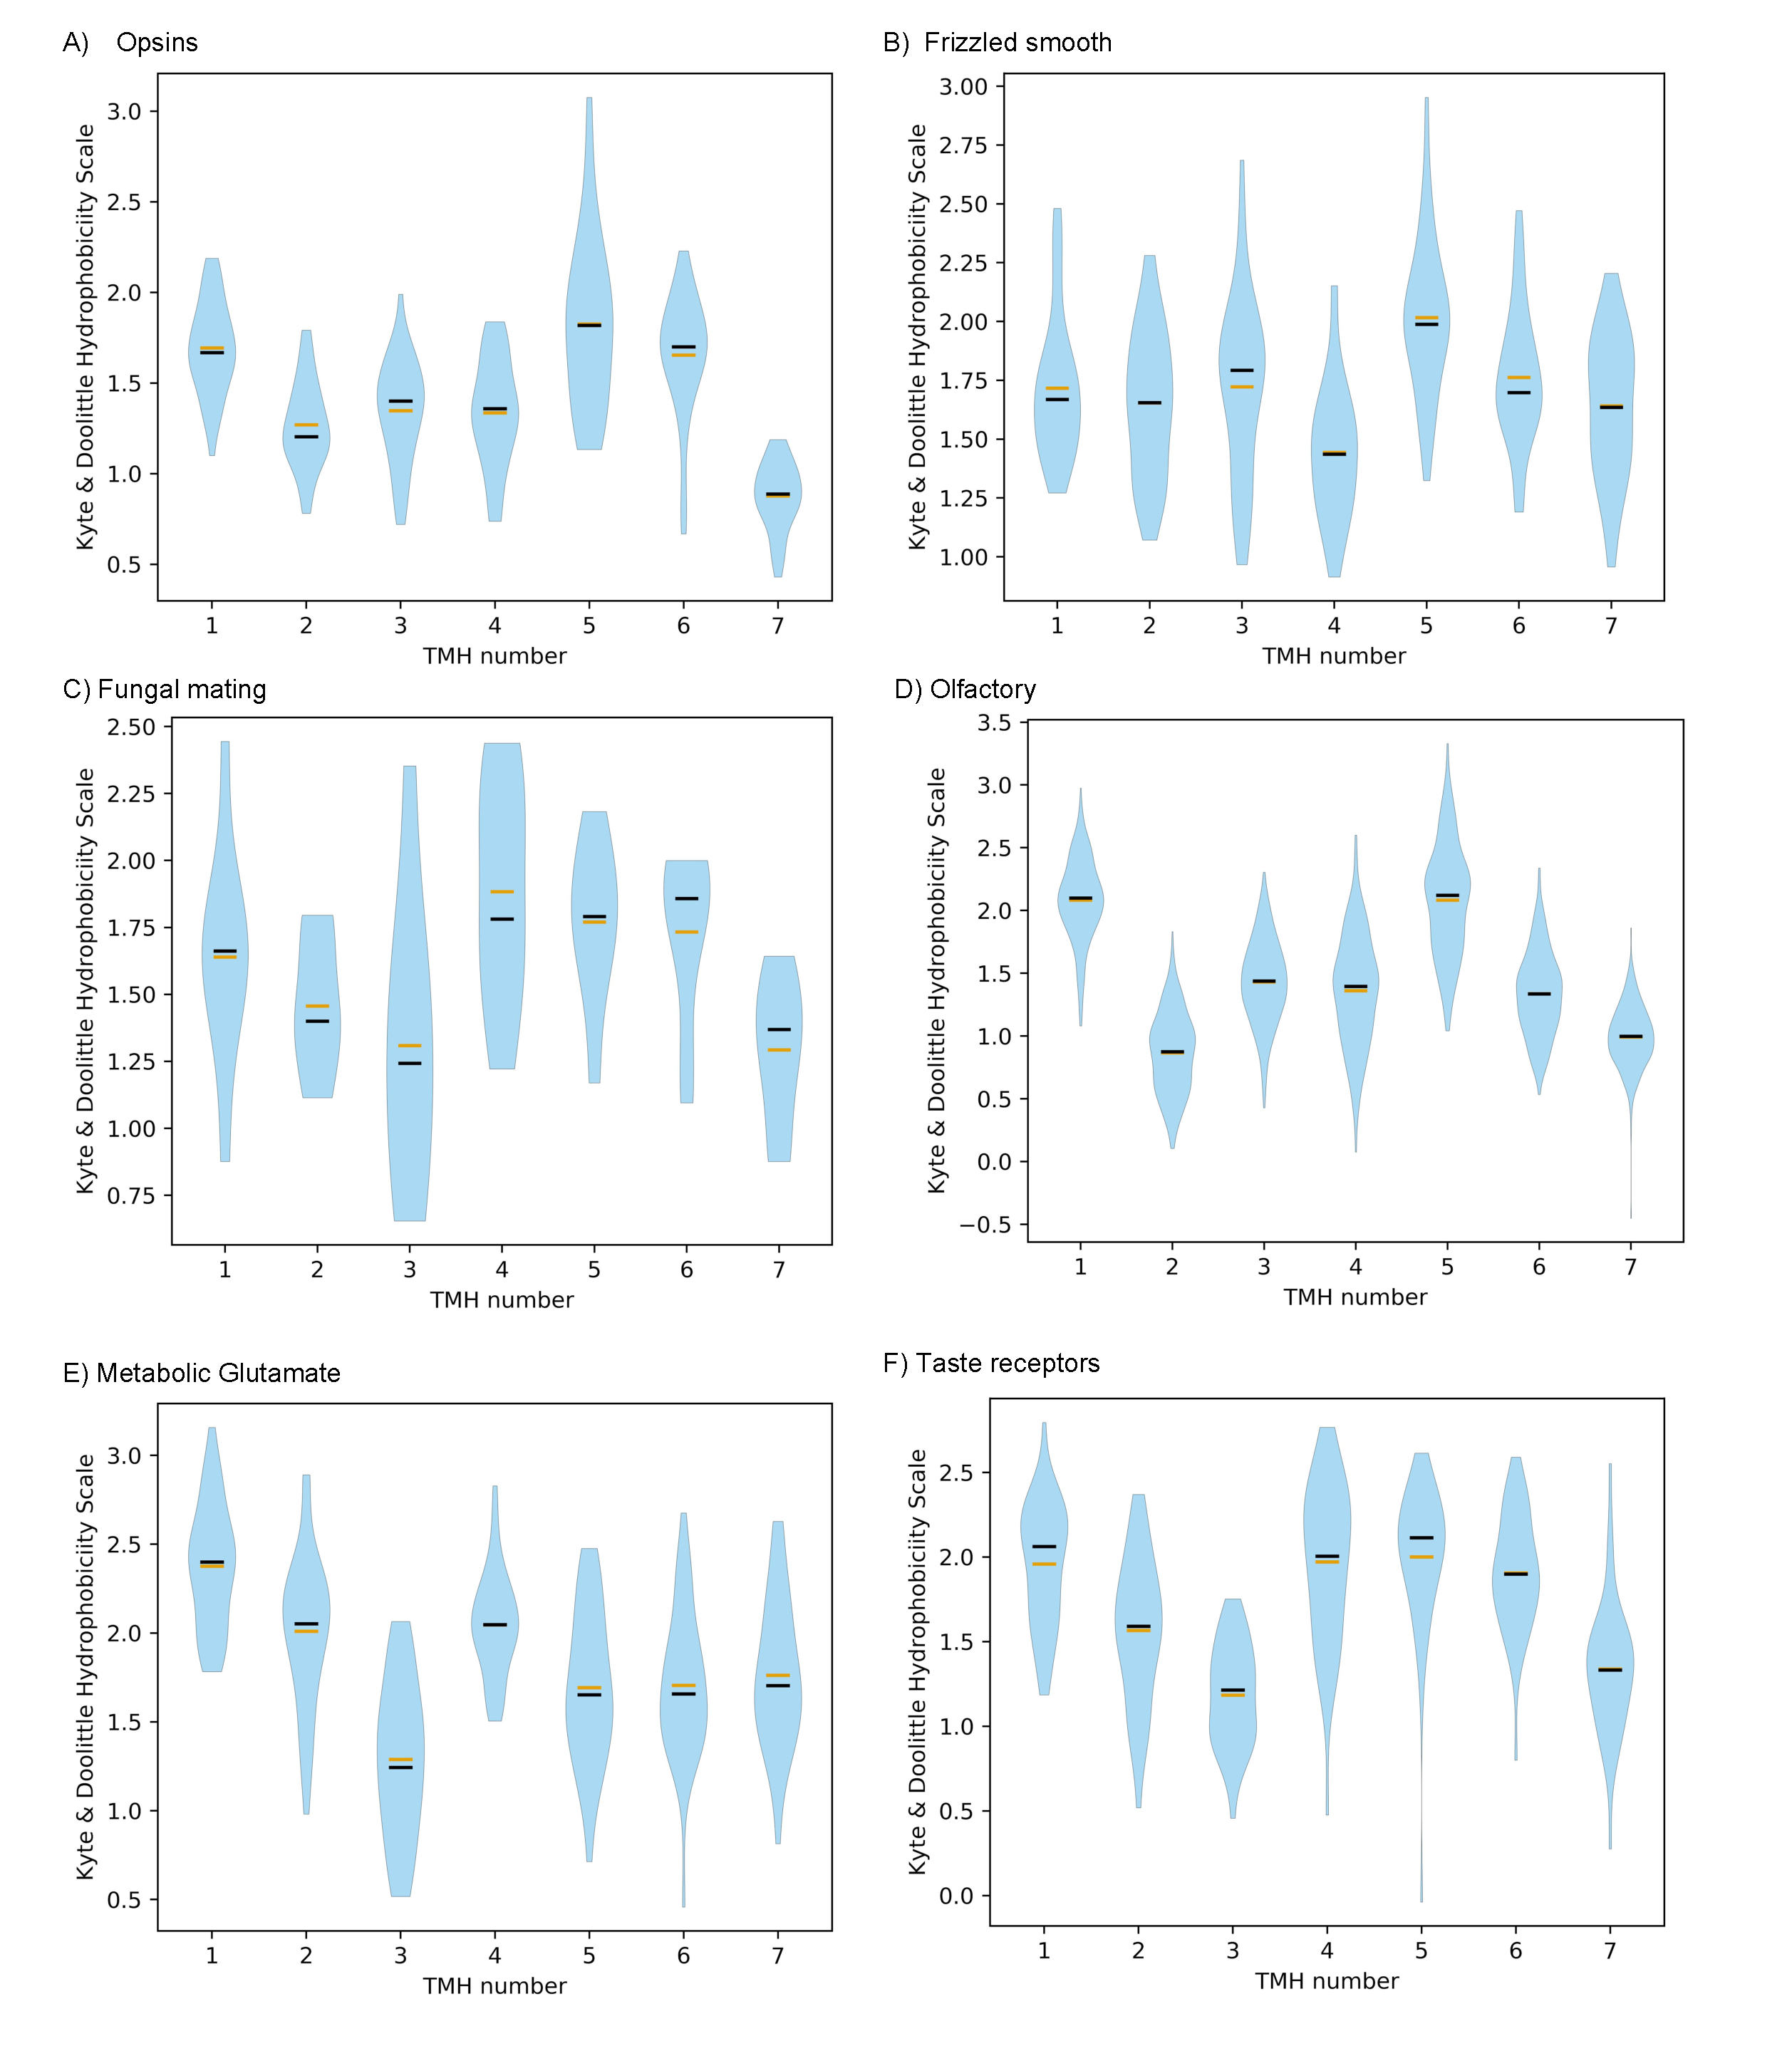
\includegraphics[width=1\textwidth]{multipass-folding/KD-GPCR}
		\captionof{figure}[The hydrophobicity of transmembrane helices in GPCR subfamilies.]{\textbf{The hydrophobicity of transmembrane helices in GPCR subfamilies.}
    Violin plots of the Kyte \& Doolittle hydrophobicity \cite{Kyte1982} of \gls{tmh}s of \gls{gpcr}s after selecting a non-exhaustive sample of \gls{gpcr} subfamilies with a wide variety of molecular functions.
    A) Opsins (N=39).
    B) Frizzled-smooth \gls{gpcr}s (N=38).
    C) Fungal mating \gls{gpcr} proteins (N=9).
    D) Olfactory receptor proteins (N=263).
    E) Metabolic glutamate receptor (N=41).
    F) T2R taste receptors (N=45)
    }

\label{fig:KD-GPCR}
\end{figure}

Opsins are a group of light\--sensitive \gls{gpcr}s that exhibit the TMH6\--TMH7 hydrophobic discrepancy (Figure \ref{fig:KD-GPCR}A).
It was shown by cross\--linking studies that opsin \gls{tmh}s 5-7 are retained in the \gls{er} translocon and only partition into the membrane once biosynthesis is complete \cite{Ismail2008}.
The timing of this partitioning is controlled by the hydrophobicity of the \gls{tmh}, not protein length or the relative position of the \gls{tmh} within the protein.
Although artificially extending the C-terminal did not result in the release of the \gls{tmh}s, by replacing native TMH7 with a more hydrophobic \gls{tmh}, the speed of insertion was decreased.
\gls{tmh}s 1-4 are inserted independently, and the 5-7 \gls{tmh}s partition into the membrane at the same time.

Since lowering the difference in hydrophobicity between TMH6 and TMH7 impedes efficient insertion of the \gls{gpcr} \cite{Ismail2008}, one would expect the terminal \gls{tmh} to be more hydrophobic rather than relatively polar \cite{Virkki2014}.
This hydrophobic difference is highly conserved throughout \gls{gpcr}s generally (Figure \ref{fig:GPCR-structures}F), and especially in many of the subfamilies(Figure \ref{fig:KD-GPCR}A, C, D, F).
We believe that the hydrophobic difference of TMH6 and TMH7 is highly important to the biogenesis of \gls{gpcr}s.
This could be evidence for widespread biologically employed \gls{tmh} cooperation during translocation of a typically hydrophobic \gls{tmh} remaining in association with the translocon until the relatively polar \gls{tmh} is processed by the insertion machinery.


\subsection{6TMH ion channels contain polar-hydrophobic transmembrane helix pairs/groups indicative of conserved cooperative insertion}

Another group of proteins that featured heavily on the list of top \gls{tmh} pairs with a high hydrophobic discrepancy was ion channels (Figure \ref{fig:good-bad-ontology}B).
Ion channels are a much more structurally varied class of \gls{tmp} than \gls{gpcr}s, varying greatly in their number of \gls{tmh}s, so a summary structural alignment equivalent to Figure \ref{fig:GPCR-structures}A, B, and C was not possible.

Voltage\--gated ion channels are another example of cooperative \gls{tmh} insertion.
The 3rd and 4th \gls{tmh} of the potassium channel (shaker family) has been shown to insert either sequentially or cooperatively \cite{Zhang2007, Cymer2015}.
This is especially notable in the case of KAT1, that is a plant K$_v$ channel that is thought to mediate long-term potassium influx into guard cells causing the stomata to open.
In the case of KAT1, N\--glycosylation of various mutant fusion KAT1 constructs revealed that there is no choice of sequential insertion since TMH3 and TMH4 have no insertion potential and no topogenic functions themselves \cite{Sato2002, Sato2003}.
In TMH4 this is due to the charged residues making it relatively polar.
However, previous experimentation in $K_{v}$1.3 had found that while TMH4 did not initiate insertion, it did have insertion potential and that when constructs contained multiple \gls{tmh}s, membrane insertion efficiency increased \cite{Tu2000}.
Without the ability to stop the translation through the translocon and form a \gls{tmh}, it was suggested that a different means was needed than classic sequential insertion, and even that TMH3 and TMH4 are integrated by the translocon at the same time post-translationally, i.e the \gls{tmh}s are folded prior to insertion \cite{Sato2003}.
They achieve this in part because the previous \gls{tmh}s,  TMH1 and TMH2, form a firm ``base'' within the membrane environment.

\begin{figure}[!ht]
\centering
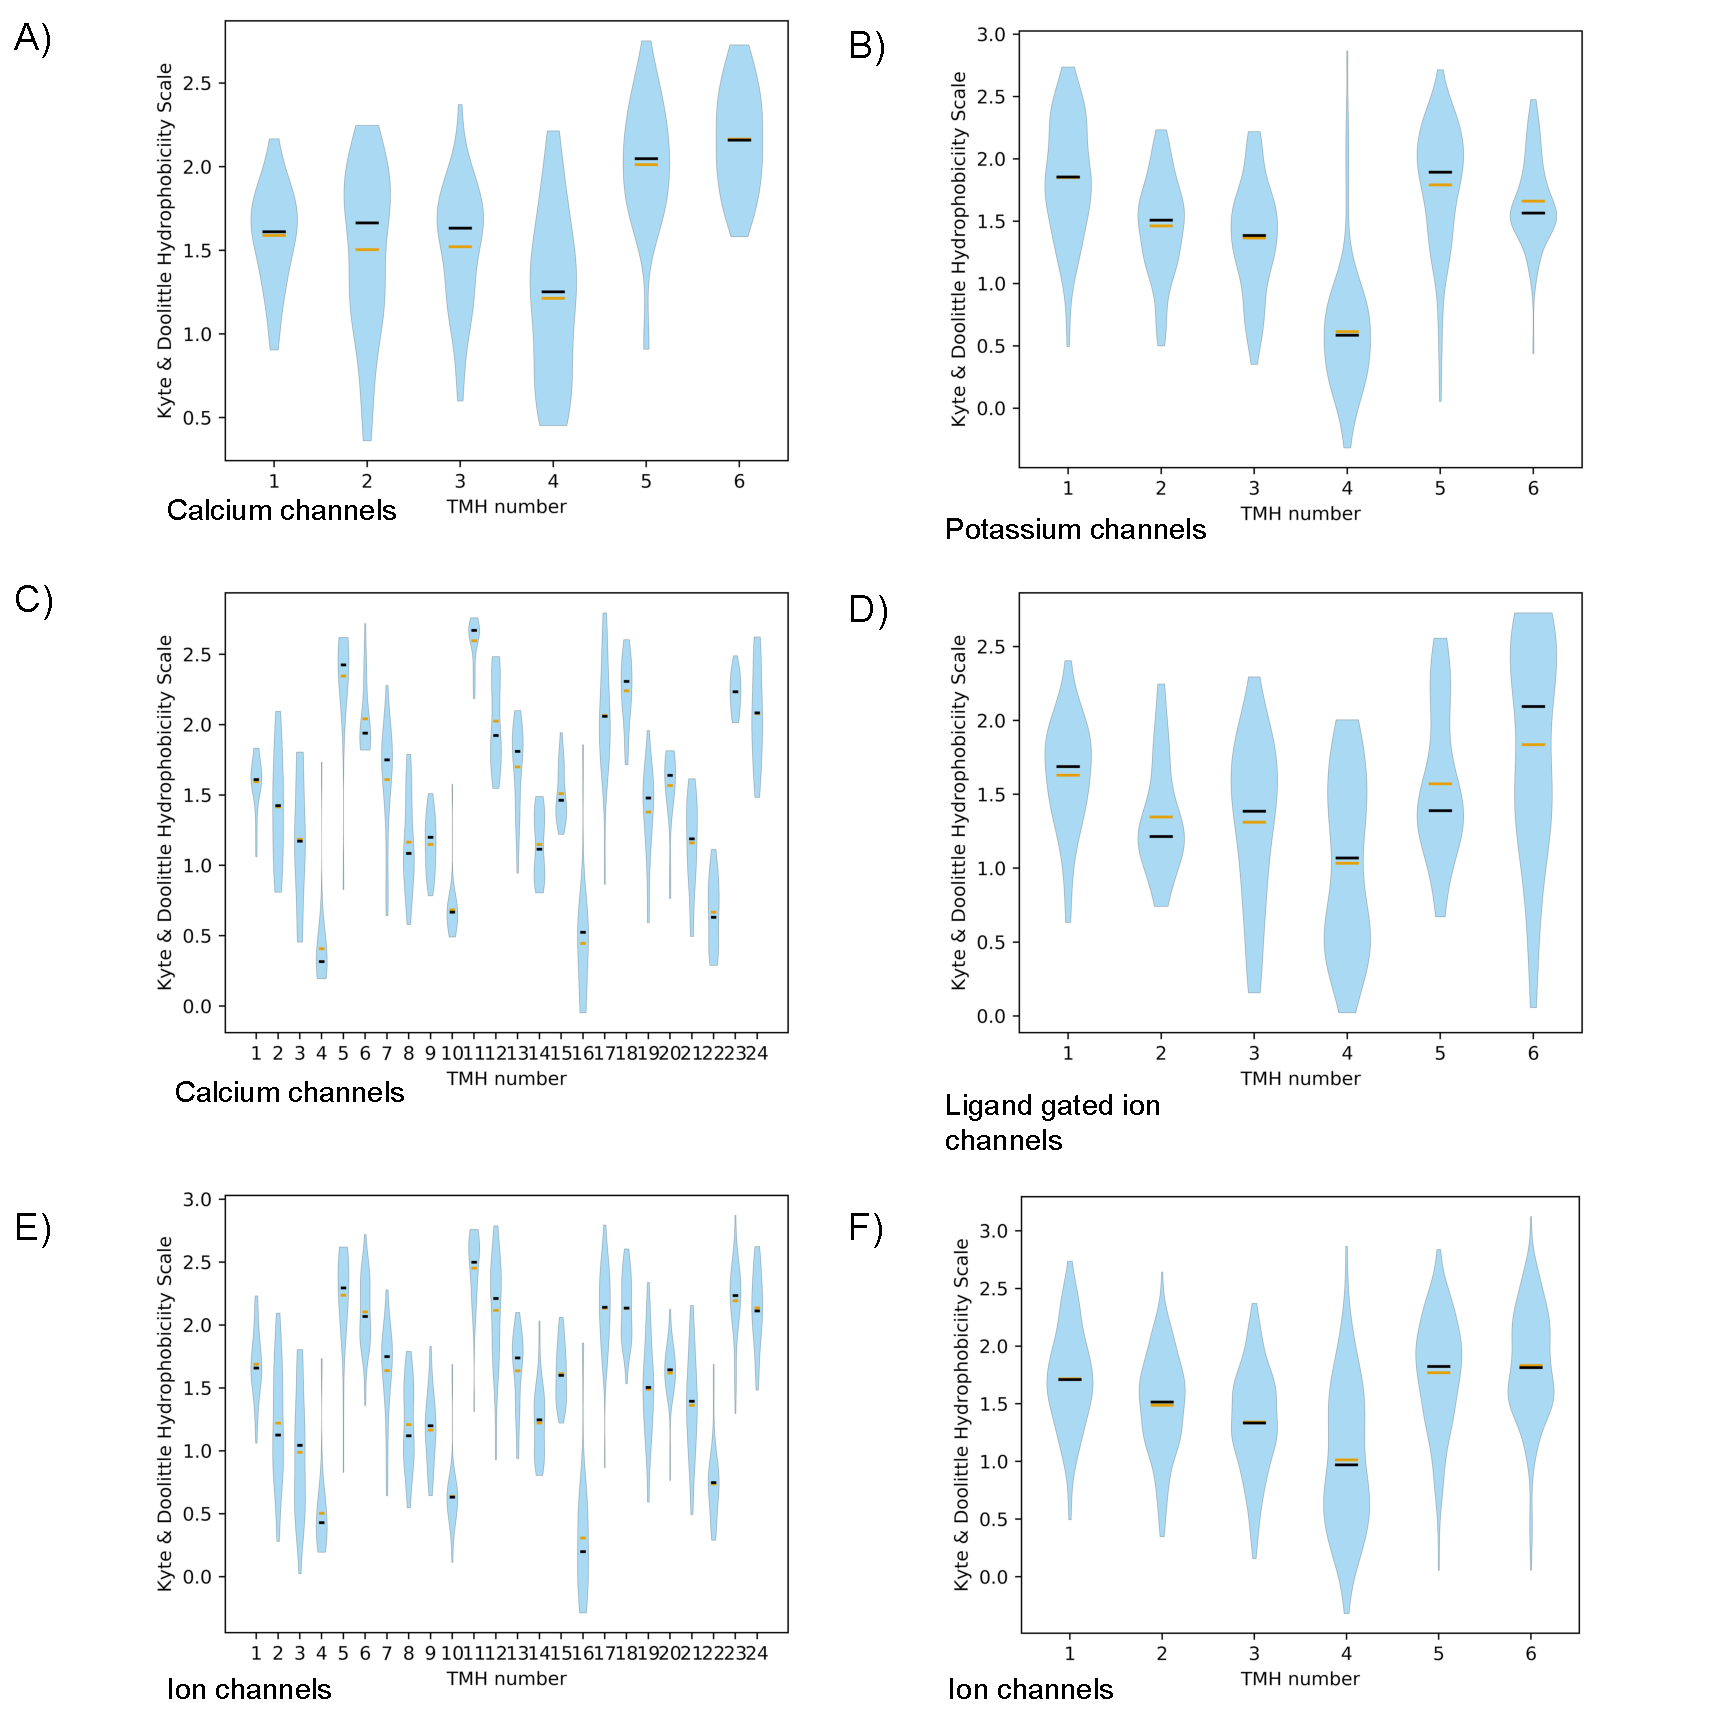
\includegraphics[width=0.9\textwidth]{multipass-folding/KD-ion-channels}
		\captionof{figure}[The hydrophobicity of transmembrane helices in ion channels.]{\textbf{The hydrophobicity of transmembrane helices in ion channels.}
    A) The Kyte \& Doolittle \gls{tmh} hydrophobicity of \gls{tmh}s according to their \gls{tmh} number of the 6TMH class of ion channels.
    N=188 (The total number of \gls{tmh}s analysed is 1128).
    The data is presented as a violin plot.
    The thickness of the bar indicates a higher density of points at that hydrophobic value.
    B) A similar violin plot as in (A), however with the 24 TMH class of ion channel.
    N=35 (A total of 840 \gls{tmh}s analysed).
    C) A subset of (A) with the keyword of ion channels restricted to voltage\--gated ion channels.
    N=97.
    D) A subset of (A) with the keyword of ion channels restricted to ligand\--gated channels.
    N=33.
    E) A subset of (A) with the keyword of ion channels restricted to calcium channels.
    N=38.
    F) A subset of (A) with the keyword of ion channels restricted to potassium channels.
    N=88.
    G) The general schematic of an ion channel.
    P indicates the pore\--forming area of the protein, which is integrated into the membrane but is not a membrane\--spanning unit.
    In the case of the 24 class, this pattern is repeated 4 times.
    }

\label{fig:KD-ion-channels}

\end{figure}

In the 6TMH class of ion channels, we observe a conserved difference in the relatively polar TMH4 known to carry charged residues (Figure \ref{fig:KD-ion-channels}A).
When using the Kyte \& Doolittle hydrophobic scale, the hydrophobic step change between TMH3 (mean hydrophobicity of 1.34) and TMH4 (mean hydrophobicity of 1.01) is statistically significantly different (Welch's t\--test P\--value = 1.83E\--8).
This is the most significant step change besides TMH4 to TMH5 (mean hydrophobicity of 1.77, Welch's t\--test P\--value = 1.88E\--31).
TMH5, the pore\--forming region, and TMH6 can be integrated independently into the membrane, but TMH3 and TMH4, at least in the case of KAT1, cannot \cite{Sato2002}.
However, there is strong evidence that TMH3 and TMH4 cooperate with one another during membrane integration and are inserted at the same time \cite{Sato2002, Sato2003, Zhang2007, Cymer2015}.
This leads us to be inclined to believe that the hydrophobic gap here that indicates a conserved cooperative role between \gls{tmh}s is that between TMH3 and TMH4 rather than TMH4 and TMH5.



This statistical difference between the hydrophobicity of TMH3 and TMH4 holds true for voltage\--gated ion channels (Welch's t\--test P\--value = 1.57E-17) (Figure \ref{fig:KD-ion-channels}C).
However, the pattern is more obscure in ligand\--gated ion channels (Welch's t\--test P\---value = 5.32E-2).
The difference does appear to match the general pattern, however, albeit as a trend, in the 33 records; there is a decrease in the mean hydrophobicity from 1.31 to 1.03 (Figure \ref{fig:KD-ion-channels}D).

 The TMH3 TMH4 hydrophobic step also appears to be independent of the ion being transported.
 For calcium ion channels the drop from TMH3 (mean hydrophobicity 1.52) to TMH3 (mean hydrophobicity 1.21) is significant (Welch's t\--test P\--value = 3.57E-3) given the relatively low sample size (38 protein records) (Figure \ref{fig:KD-ion-channels}E).
In potassium channels, the difference is even greater between TMH3 (mean hydrophobicity of 1.37) and TMH4 (mean hydrophobicity of 0.61) (Welch's t\--test P\--value = 2.52E-19) in potassium ion channels (Figure \ref{fig:KD-ion-channels}F).

The observed difference between TMH3 and TMH4 is somewhat independent of the scale chosen (Figure \ref{fig:ion-channel-hydrophobicity-verification}), however, the Kyte \& Doolittle scale is the most sensitive to the hydrophobic differences between TMH3 and TMH4.
Statistical significance was found in the difference between TMH3 and TMH4 in the Eisenberg scale (Welch's t\--test P\--value = 4.74E-23), the White and Wimley scale (Welch's t\--test P\--value = 1.26E-3).
The Hessa/von Heijne biological scale was particularly insensitive to the mean difference (Welch's t\--test P\--value = 7.56E-2), but can scrutinise some difference in the skews of the data (Kolmogorov Smirnov test  P\--value = 1.56E-4, Kruskal Wallis P\--value = 4.00E-2) indicating that whilst biophysically the \gls{tmh}s are distinct, the translocon may not readily scrutinise the hydrophobicity between the two.
All the scales however corroborate the large hydrophobic difference between TMH4 and TMH5 (Welch's t\--test P\--values for Hessa = 1.23E-35, White and Wimley = 4.82E-23, Eisenberg = 5.72E-41)

\begin{figure}[!ht]
\centering
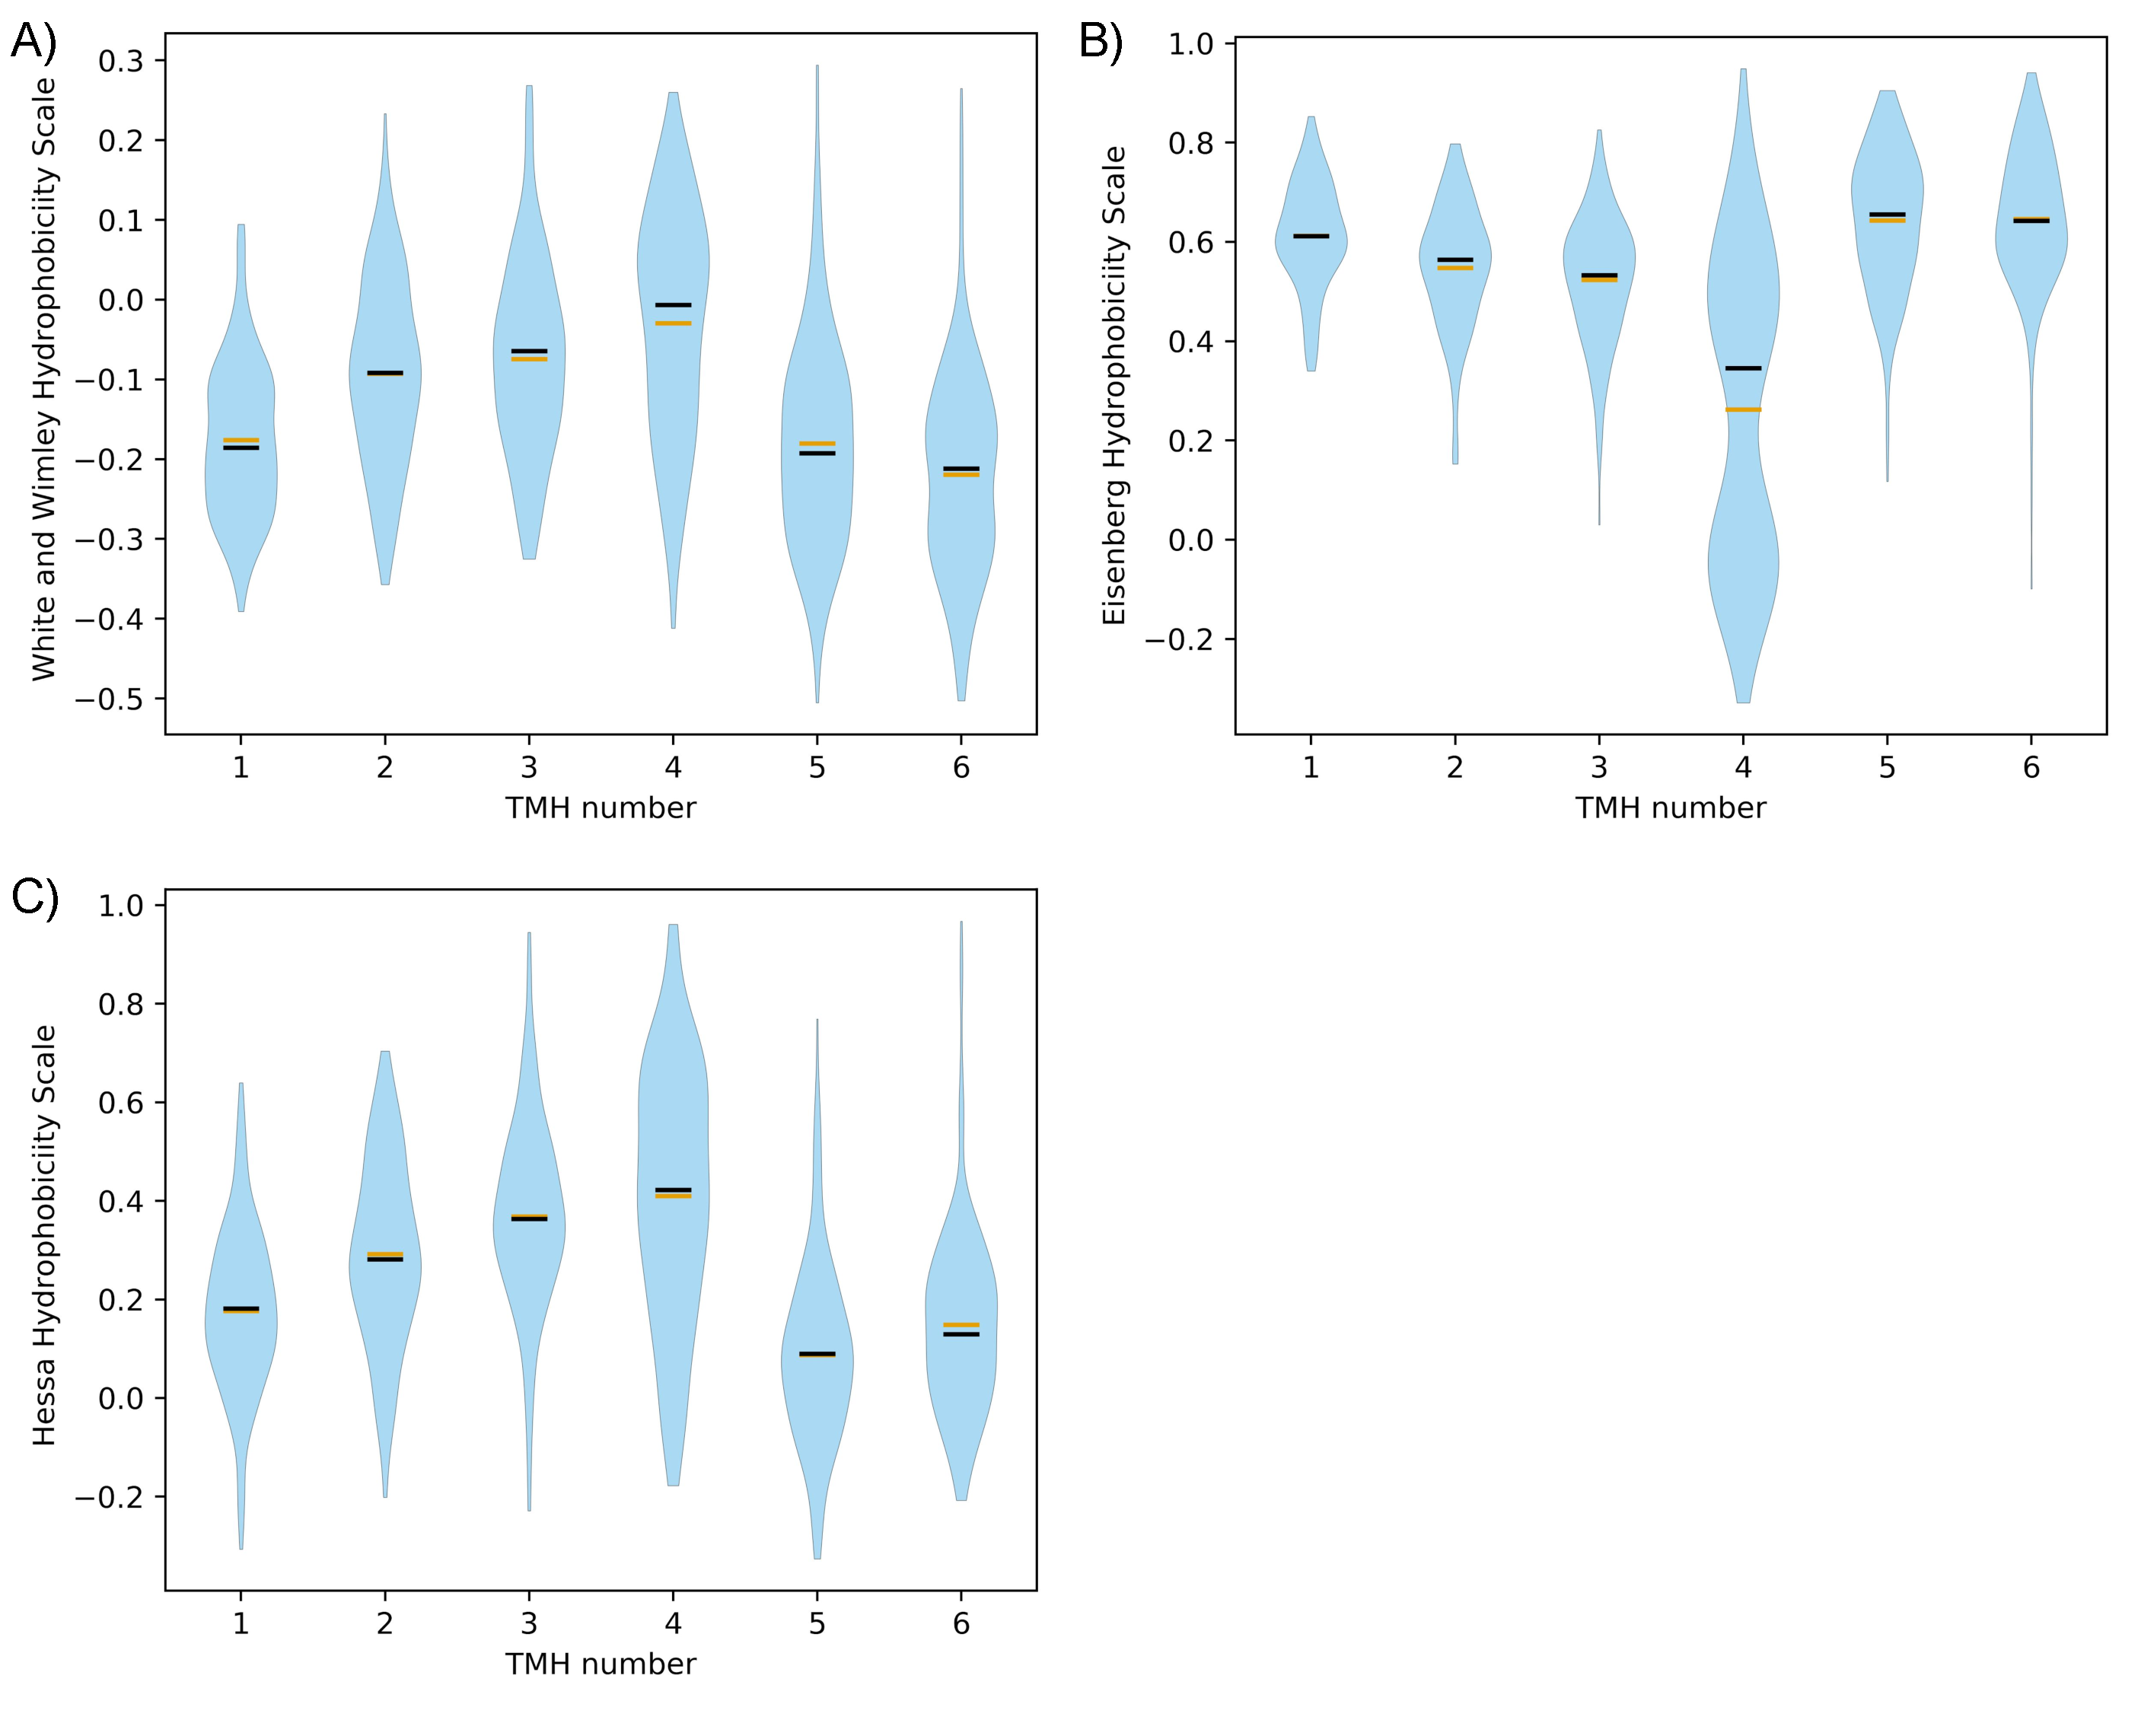
\includegraphics[width=1\textwidth]{multipass-folding/ion-channel-hydrophobicity-verification}
  \captionof{figure}[The hydrophobic difference observed between TMH4 and the neighbouring transmembrane helices in 6TMH ion channels is not due to the choice of hydrophobic scale.]{\textbf{The hydrophobic difference observed between TMH4 and the neighbouring transmembrane helices in 6TMH ion channels is not due to the choice of hydrophobic scale.}
  Three different scales were applied to the same dataset used in figure \ref{fig:KD-ion-channels}A to verify the observed differences were not caused by the choice of scale.
  A) The White and Wimley biophysical scale \cite{White1999}
  B) The Eisenberg consensus scale \cite{Eisenberg1984}.
  C) The von Heijne/Hessa biological scale \cite{Hessa2005}.}

\label{fig:ion-channel-hydrophobicity-verification}
\end{figure}

24TMH class is essentially a modular variant of the 6TMH class, and has even more extreme discrepancies between the equivalent 4 TMHs (Figure \ref{fig:KD-ion-channels}B).
In the first cluster, TMH3 (mean Kyte \& Doolittle hydrophobicity = 0.96) to TMH4 (mean hydrophobicity = 0.47) is different (Welch's t\--test P\--value = 5.16E-6), but even more so is the step up from TMH4 to TMH5 (hydrophobicity = 2.26, Welch's t\--test P\--value = 5.16E-32).
The preceding step is weaker, and the proceeding step is greater throughout the 6TMH ``modules''.
A similar step change is found between TMH9 and TMH10 (P\--value = 3.02E-13) and TMH10 to TMH11 (P\--value = 5.51E-44), TMH15 to TMH16 (P\--value = 1.79E-23), TMH16 to TMH17 (P\--value = 1.67E-27), TMH21 to TMH22 (P\--value = 1.64E-9), and TMH22 to TMH23 (P\--value = 3.42E-31).

Oddly, as a trend, the TMSOC  z\--score was not sensitive to detecting function in the extremely hydrophobic TMH4 (Figure \ref{fig:Ion-channel-information-entropy}).
This is due to the other component of the  z\--score, the sequence information entropy \cite{Wong2011, Wong2012}.
The relative probability of a polar/charged residue is so high in TMH4 that it apparently has the same expectancy as the hydrophobic residues, and the ``simple'' entropy mutes somewhat the effect of the extreme hydrophobicity.
This is compounded by the fact that the White and Wimley scale (used to generate the  z\--score) is already less sensitive to the relative polarity difference between TMH3 and TMH4 than the Kyte \& Doolittle scale (Figure \ref{fig:KD-ion-channels}A, Figure \ref{fig:ion-channel-hydrophobicity-verification}A).

\begin{figure}[!ht]
\centering
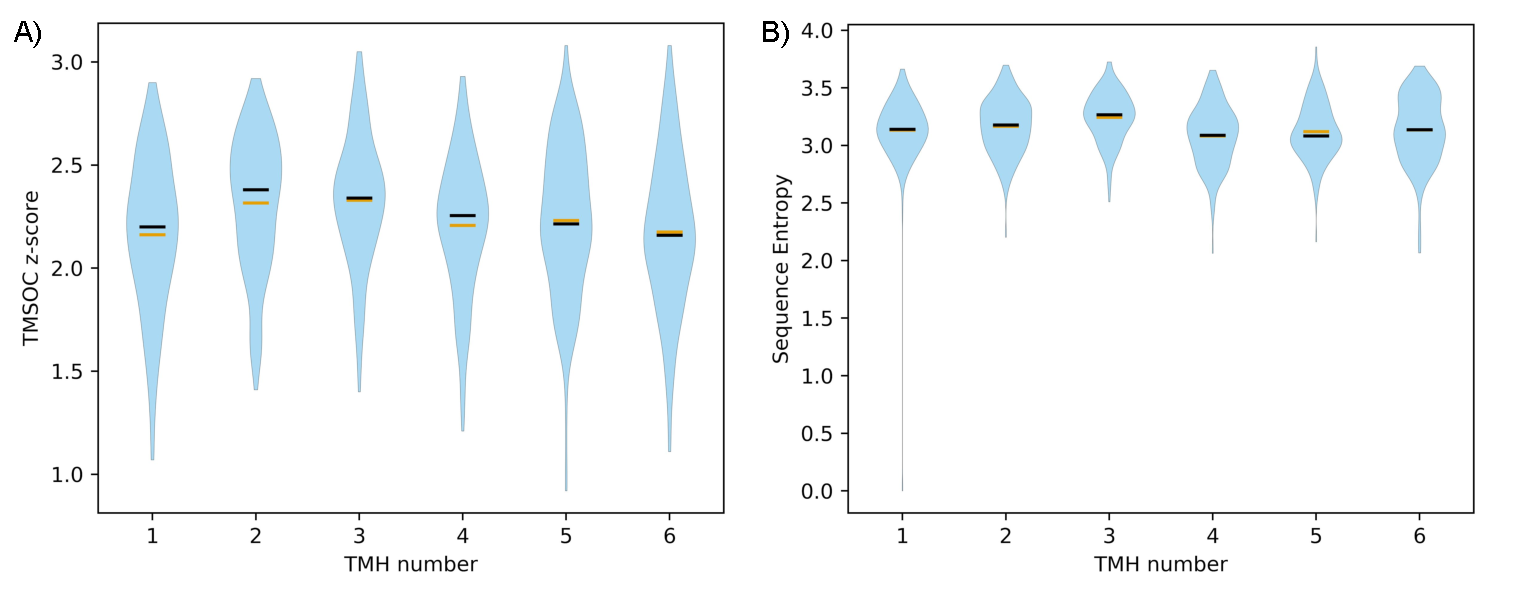
\includegraphics[width=1\textwidth]{multipass-folding/Ion-channel-information-entropy}
		\captionof{figure}[Sequence entropy is unsuitable for assessing function in TMH4 of ion channels.]{\textbf{Sequence entropy is unsuitable for assessing function in TMH4 of ion channels.}
    A) The TMSOC  z\--score \cite{Wong2011, Wong2012} of \gls{tmh}s from the ion channel dataset used in Figure \ref{fig:KD-ion-channels}A.
    B) The sequence information entropy of those same \gls{tmh}s.
    }

\label{fig:Ion-channel-information-entropy}
\end{figure}


\subsection{The prevalence of the high hydrophobic discrepancy of transmembrane helices amongst other common ``transporter'' transmembrane protein classes.}

Whilst the gene ontology recognises ``transporters'' as having disproportionately more highly different hydrophobic sequential pairs, the list is predominantly ion channels, which are molecularly and functionally different from ion transporters.
It also appears that ion transporters have no conserved hydrophobicity discrepancy between any of their \gls{tmh}s for the 4TMH, 6TMH, 8TMH, or 10TMH classes (Figure \ref{fig:other-groups-good-bad} C, D, E, F, G).

\begin{figure}[!ht]
\centering
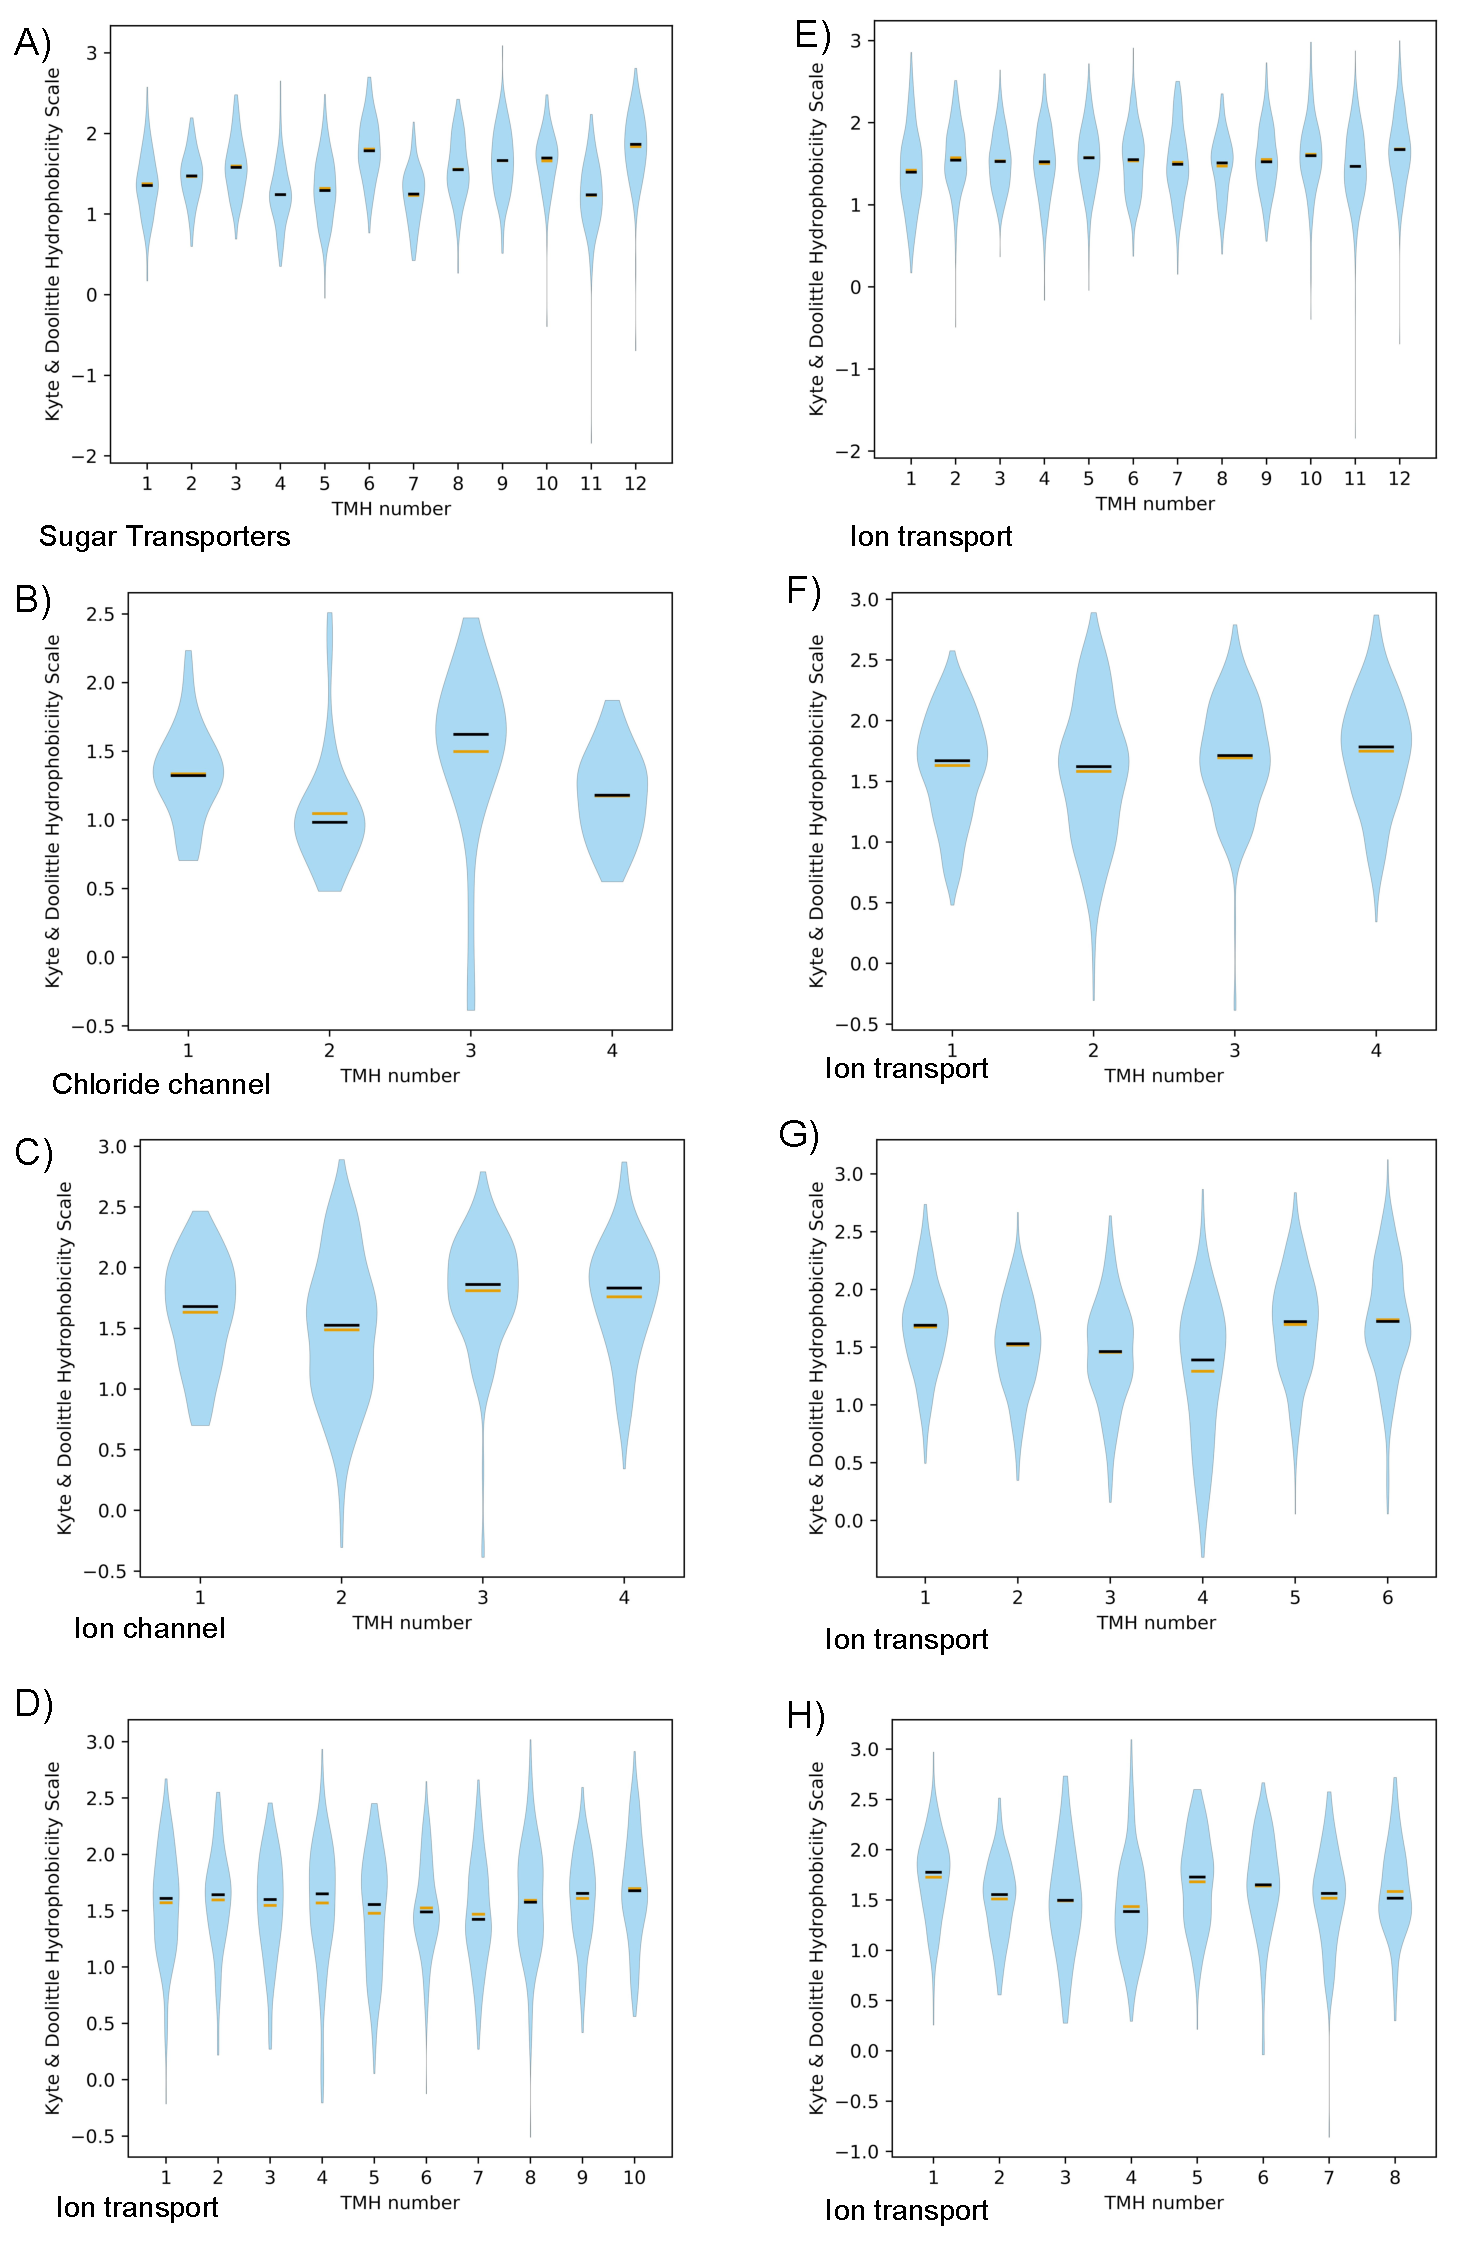
\includegraphics[width=0.8\textwidth]{multipass-folding/other-groups-good-bad}
		\captionof{figure}[High polarity discrepancy between sequentially adjacent transmembrane helices is not present in all transmembrane protein transporter families.]{\textbf{High polarity discrepancy between sequentially adjacent transmembrane helices is not present in all transmembrane protein transporter families.}
    The mean average Kyte \& Doolittle hydrophobic scores of a \gls{tmh}s from various families and classes of membrane transporter proteins.
    Datasets are represented as a violin plot where thickness denotes the relative density of the population distribution.
    A) A dataset of  134 sugar transporters containing 12 \gls{tmh}s.
    B) A dataset of 50 chloride channels containing 4 \gls{tmh}s.
    C) 234 ion channels with 4 \gls{tmh}s.
    D-H) Ion transporters restricted to the number of \gls{tmh}s on the horizontal axis.
    Sample sizes can be found in table \ref{table:datasetsizes}}

\label{fig:other-groups-good-bad}
\end{figure}

Another large family of transporters are the sugar transporters.
In terms of the hydrophobic discrepancy between sequentially adjacent \gls{tmh} pairs, sugar transporters also have a few peaks and dips at TMH6 and TMH11 (Figure \ref{fig:other-groups-good-bad}A).
TMH5 (mean hydrophobicity = 1.32) to TMH6 (mean hydrophobicity = 1.81) (Welch's t\--test P\---value = 3.09E-19) was less significant than TMH6 to TMH7 (mean hydrophobicity = 1.23) (Welch's t\--test P\--value = 8.75E-29).
TMH10 (mean hydrophobicity = 1.66) to TMH11 (mean hydrophobicity = 1.23) (Welch's t\--test P\--value = 1.03E-14) was also less significant than TMH11 to TMH12 (mean hydrophobicity = 1.84) (Welch's t\--test P\--value = 3.22E-22).

The ion channel 4TMH class also has a discrepancy between TMH2 (Kyte \& Doolittle hydrophobicity = 1.49) and TMH3 (hydrophobicity = 1.81) (Welch's t\--test P\---value = 4.42E-10, from 234 records) (Figure \ref{fig:other-groups-good-bad}C).
The largest family within the 4TMH class is the chloride channel 4TMH family.
A jump of hydrophobicity is observed in TMH2 (hydrophobicity = 1.05) to TMH3 (hydrophobicity = 1.50) (Welch's t\--test P\---value = 5.34E-5, from 50 records) (Figure \ref{fig:other-groups-good-bad}B).

\section{Summary}

Marginally hydrophobic \gls{tmh}s are often essential physiological components for carrying out complex intra-membrane tasks beyond membrane anchorage, and widely prevalent among \gls{tmp}s \cite{Hessa2007}.
However, this presents a significant biophysical and biological challenge; how to incorporate and maintain such necessarily relatively polar \gls{tmh}s into the membrane.
We show that among certain classes of \gls{tmp}s that this is a conserved issue.
It was recently discovered that the \gls{emc} protein assists the translocon with the marginally hydrophobic \gls{tmh}s, particularly those containing charged residues  \cite{Shurtleff2018}.
There is also evidence to suggest that multipass \gls{tmh} arrangements work cooperatively during translocation and insertion to achieve correct folding of marginally hydrophobic \gls{tmh}s \cite{Ismail2008, Virkki2014, Sadlish2005, Cross2009, Cymer2013, Sato2002, Sato2003, Zhang2007, Cymer2015, Tu2000, Tu2014, Ojemalm2012} (Figure \ref{fig:Good-bad-TMH}).

\begin{figure}[!ht]
\centering
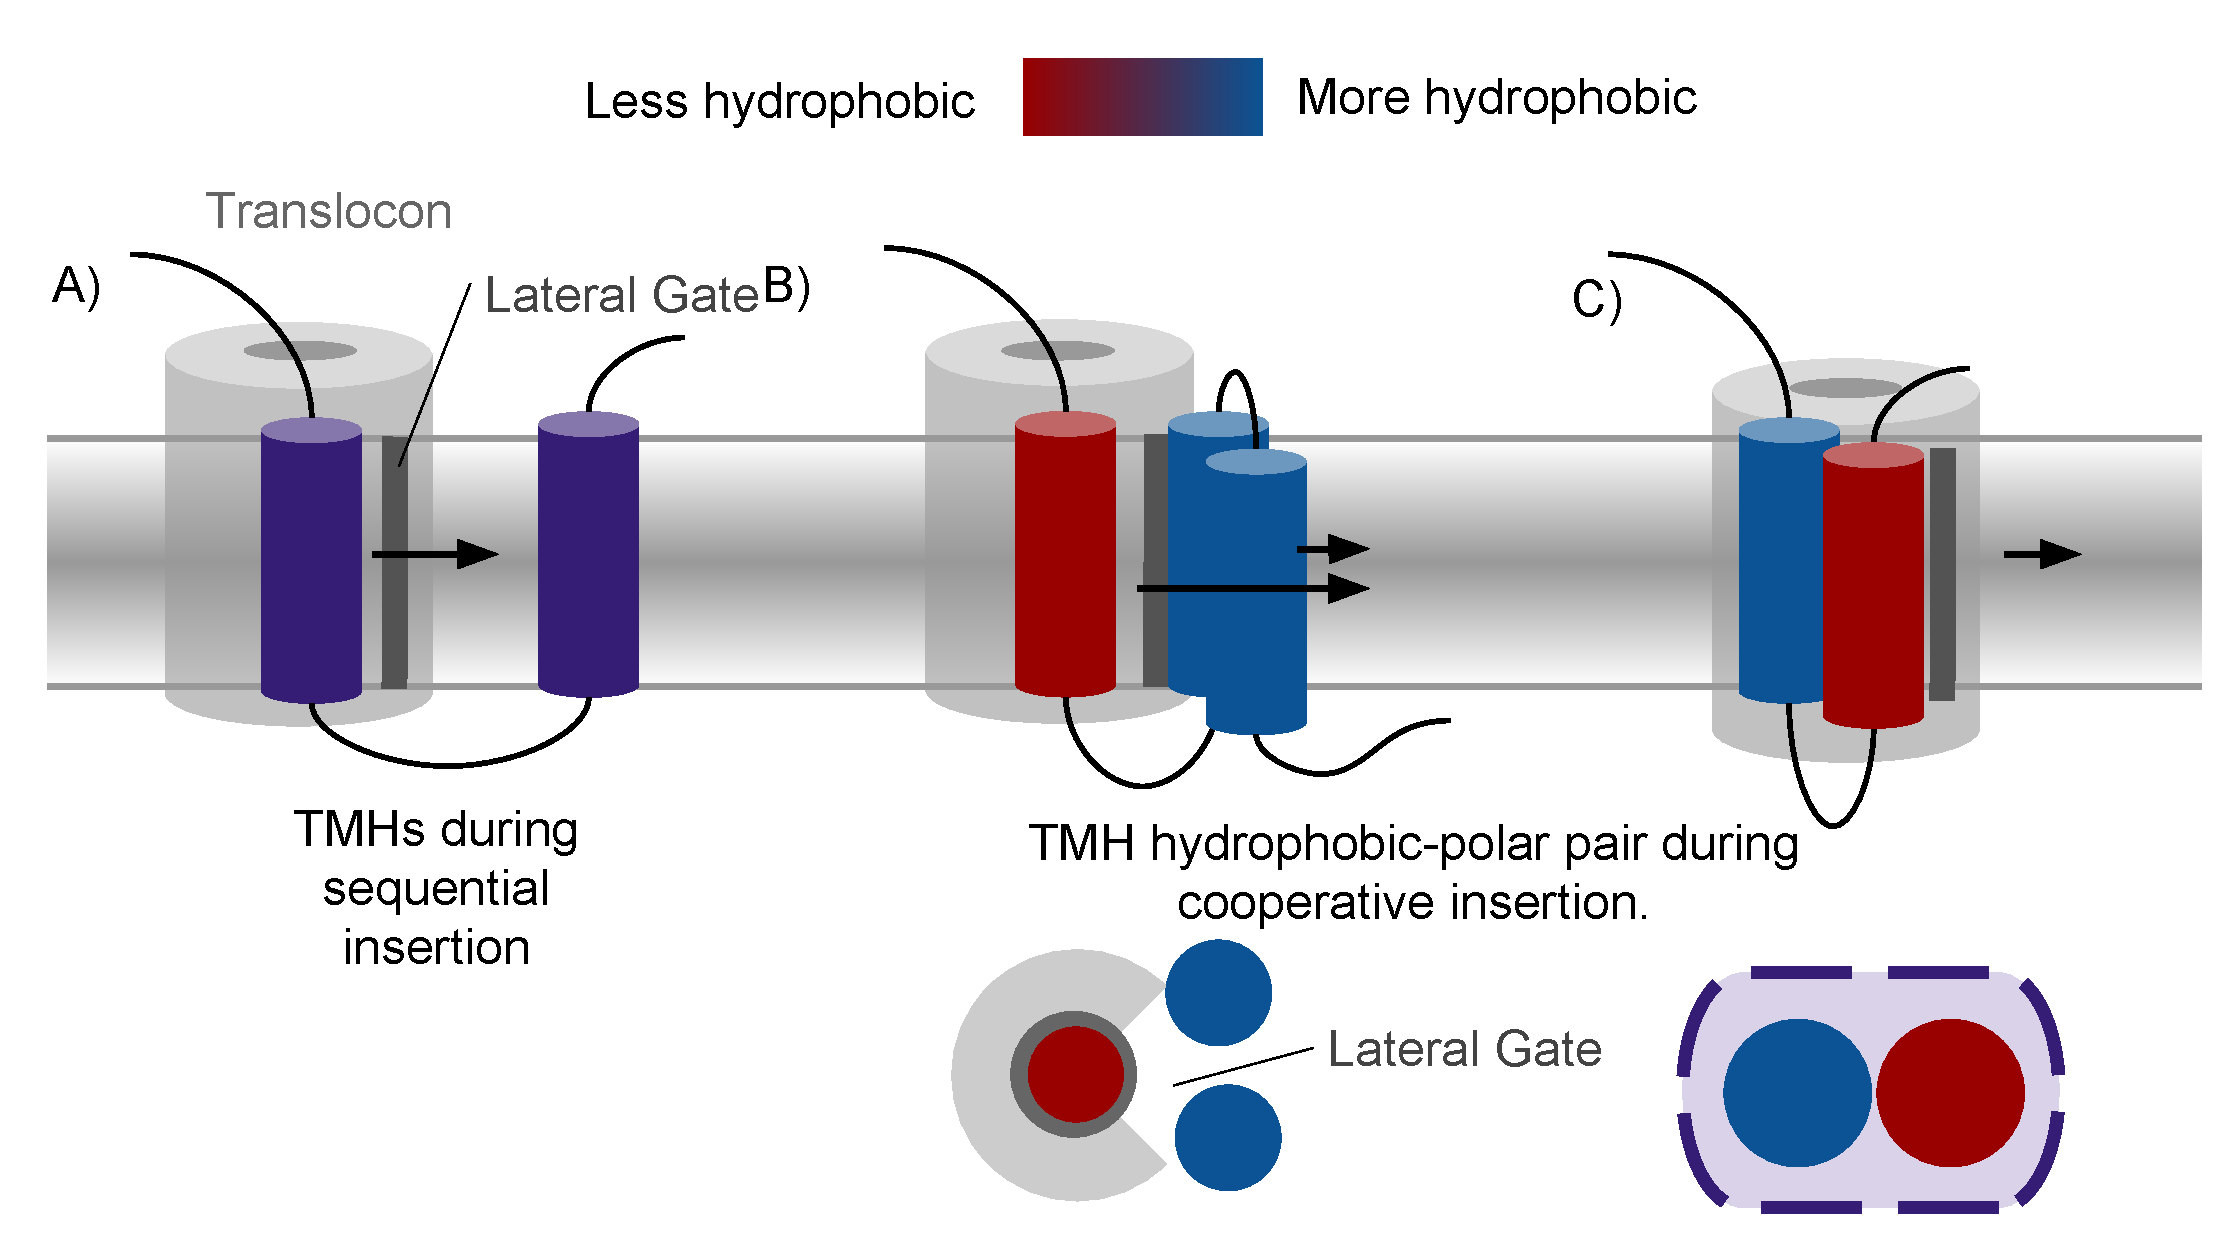
\includegraphics[width=1\textwidth]{multipass-folding/Good-bad-TMH}
		\captionof{figure}[A cartoon of potential cooperative transmembrane helix insertion methods.]{\textbf{A cartoon of potential cooperative transmembrane helix insertion methods.}
    A) Typically hydrophobic \gls{tmh}s remain in association with the translocon machinery until the marginally hydrophobic \gls{tmh} is released into the membrane.
    This was observed in an opsin protein \cite{Ismail2008}.
    B) \gls{tmh}\--\gls{tmh} interactions allow the marginally hydrophobic \gls{tmh} to shield the polar residues.
    The marginally hydrophobic \gls{tmh} can associate with the typical hydrophobic \gls{tmh} in the ribosomal exit tunnel \cite{Tu2014} or in the translocon tunnel \cite{Zhang2007}.
    This was observed in a potassium ion channel \cite{Tu2014, Zhang2007, Cymer2015}.
    }

\label{fig:Good-bad-TMH}
\end{figure}

Here, we have shown that high discrepancy of TMSOC  z\--score (simple-complex score) \cite{Wong2011, Wong2012}, and several hydrophobicity scales \cite{Hessa2005, Kyte1982, White1999, Eisenberg1984}, between sequentially adjacent \gls{tmh}s corroborates \gls{tmh} groups known to insert cooperatively \cite{Ismail2008, Sato2003, Zhang2007, Cymer2015}.
The hydrophobic relationships between these cooperatively inserted \gls{tmh}s may be conserved throughout their larger families indicating that cooperative insertion may be a routine mechanism for the insertion of some families of \gls{tmp}s.
So far, this method has shown that the TMH7 of \gls{gpcr}s is a conserved marginally hydrophobic \gls{tmh} with the typically hydrophobic TMH6 preceding it.
In opsins, TMH5\--TMH7 are incorporated into the membrane together simultaneously by staying in association with the translocon until TMH7 emerges \cite{Ismail2008}.
We see this pattern across several \gls{gpcr} sub\--families and the \gls{gpcr} family as a whole.
Furthermore, we found that the charged TMH4 of 6TMH ion channels has a typically hydrophobic TMH3 preceding it and a more hydrophobic TMH5 following it.
Indeed there is evidence that TMH3 and TMH4 cannot incorporate alone \cite{Sato2003}, that TMH3 and TMH4 can insert as a pair from the translocon simultaneously \cite{Zhang2007, Cymer2015}.

With the emergence of advanced cross\--linking experiments and \gls{ap}s that can probe energetics and \gls{tmh}\--\gls{tmh} interactions dynamically during ribosomal translation and membrane insertion, it could be possible to expore \gls{tmh}\--\gls{tmh} relationships in more detail.
We suggest that \gls{tmh}s with highly contrasting hydrophobicity and TMSOC z\--score could yield interesting examples of cooperative insertion during translocation.
For example, here we find discrepancies in the TMH6 and TMH11 to their adjacent \gls{tmh}s of sugar transporters as well as TMH2 and TMH3 in ion channels, specifically in chloride channels.
Understanding the biogenesis of proteins is essential to solving misfolding in disease phenotypes and for developing viable \gls{tmp} chassis in synthetic biology.
